\documentclass[17pt,a4paper]{extarticle}
\usepackage{xcolor}
\usepackage{tikz}
\usepackage[utf8]{inputenc}
\usepackage[a4paper,margin=2.5cm]{geometry}
\usepackage{setspace}
\setstretch{1.0}
\usepackage{microtype}
\usepackage{times}
\usepackage{amsmath}
\usepackage{graphicx}
\usepackage{booktabs}
\let\Bbbk\relax
\usepackage{amsmath,amssymb,amsfonts}
\usepackage{subcaption}
\usepackage{float}
\usepackage{array}
\usepackage{pifont}
\usepackage[numbers]{natbib}
\usepackage{algorithm}
\usepackage{algpseudocode}
\usetikzlibrary{calc}
\usepackage{url}
\usepackage{tocloft}
\renewcommand{\contentsname}{\LARGE\textbf{Table of Contents}} % Big bold title
\setlength{\cftbeforesecskip}{6pt} % spacing between sections
\setlength{\cftaftertoctitleskip}{1cm} % space after title
\pagestyle{plain}
\pagenumbering{arabic}

\begin{document}  % <<< START DOCUMENT HERE

% --- FRONT PAGE INFO ---
% --- FRONT PAGE INFO (Stylised) ---
% Add this to your preamble if not already present

\begin{titlepage}

\begin{tikzpicture}[remember picture,overlay]

% Outer border
\draw[line width=2pt,color=blue!60!black]
($(current page.north west)+(1.5cm,-1.5cm)$)
rectangle
($(current page.south east)+(-1.5cm,1.5cm)$);

% Inner border
\draw[line width=0.8pt,color=gray!60]
($(current page.north west)+(1.8cm,-1.8cm)$)
rectangle
($(current page.south east)+(-1.8cm,1.8cm)$);

\end{tikzpicture}

\centering

\vspace*{2cm}

{\Large \textcolor{gray!70}{COURSE PROJECT REPORT}}

\vspace{1.5cm}

{\fontsize{30}{34}\selectfont
\textbf{\textcolor{blue!70!black}{SVD-Based Noise Reduction}}\\[0.3cm]
\textbf{\textcolor{blue!70!black}{in EEG Signals}}
}

\vspace{1.2cm}

{\large \textit{22MAT230 – Mathematics for Computing}}

\vspace{2cm}

{\Large \textbf{\textcolor{blue!80!black}{Amrita Vishwa Vidyapeetham}}}

\vspace{0.2cm}


{\large Academic Year 2026}

\vspace{1.8cm}

{\large \textbf{\textcolor{red!70!black}{Team D–9}}}

\vspace{0.8cm}

\renewcommand{\arraystretch}{1.5}
\begin{tabular}{ll}
\textbf{B. Sainath Reddy} & CB.SC.U4AIE24309 \\
\textbf{K. Pushpak Siva Sai} & CB.SC.U4AIE24328 \\
\textbf{P. Manohar} & CB.SC.U4AIE24339 \\
\textbf{P. Sai Mrudula} & CB.SC.U4AIE24340 \\
\end{tabular}

\vspace{0.5cm}

{\large March 2026}

\end{titlepage}

\newpage
\tableofcontents
\newpage
\section{Abstract}
Electroencephalographic (EEG) signals are frequently contaminated by ocular artifacts,
primarily electrooculogram (EOG) signals generated by eye movements and blinks. These
artifacts obscure underlying neural activity and significantly compromise the reliability of
downstream EEG analysis. This study implements a signal processing framework based on
Singular Value Decomposition (SVD) to effectively attenuate EOG artifacts in real EEG
recordings. By exploiting the approximate orthogonality between neural and ocular sources,
the proposed SVD approach isolates and removes artifact components within the singular
value domain.

Multi-channel data matrices were constructed using contaminated EEG channels alongside one
or two dedicated EOG reference channels. SVD was applied to these matrices, projecting the
data into a transformed subspace where the clean EEG signal could be accurately
reconstructed. The experiment was conducted using our own custom-recorded EEG data,
where signals from the F3 and F4 electrodes were processed using the AF3 and AF4 channels
as EOG references.

The effectiveness of the proposed approach is evaluated using time-domain signal analysis
and Linear Prediction (LP) spectral estimation. The structural evaluation confirms that the
SVD-based method robustly minimizes ocular interference while preserving the essential
morphological and spectral characteristics of the original EEG signals, establishing it as a
highly reliable preprocessing technique for advanced neural signal enhancement.

\section{Introduction}

Electroencephalography (EEG) is a non-invasive technique utilized to measure the
electrical activity of the brain via electrodes placed on the scalp. While widely
adopted in clinical diagnostics, cognitive neuroscience, and brain-computer
interface (BCI) research, EEG signals possess inherently small amplitudes-typically
in the microvolt range. This low amplitude renders them highly susceptible to
contamination from various physiological artifacts. Among these, the
electrooculogram (EOG), generated by eye movements and blinks, represents one of
the most significant sources of signal interference.

Physiologically, the human eye acts as an electrical dipole, with the comea carrying
a positive charge relative to the retina. When the eyes move or blink, this dipole
generates substantial electrical potentials that propagate through cranial tissues to
the scalp electrodes via volume conduction. Consequently, EOG artifacts are not
localized to the ocular region; they spread across a large portion of the scalp,
appearing simultaneously across multiple EEG channels. These ocular artifacts often
exhibit amplitudes magnitudes larger than the underlying neural signals,
disproportionately affecting electrodes situated in the frontal region.

A fundamental assumption in signal separation methodologies is the statistical
independence of physiological sources. In the context of EEG analysis, this implies
that neural activity originating within the brain and ocular activity driven by eye
movements arise from distinet physiclogical mechanisms. Operating under this
assumption, recorded EEG data can be mathematically modeled as a linear mixture
of these independent sources. Therefore, the primary objective of artifact removal
techniques is to effectively disentangle and eliminate the ocular source
contributions from the neural data.
\begin{figure}[!h]
\centering
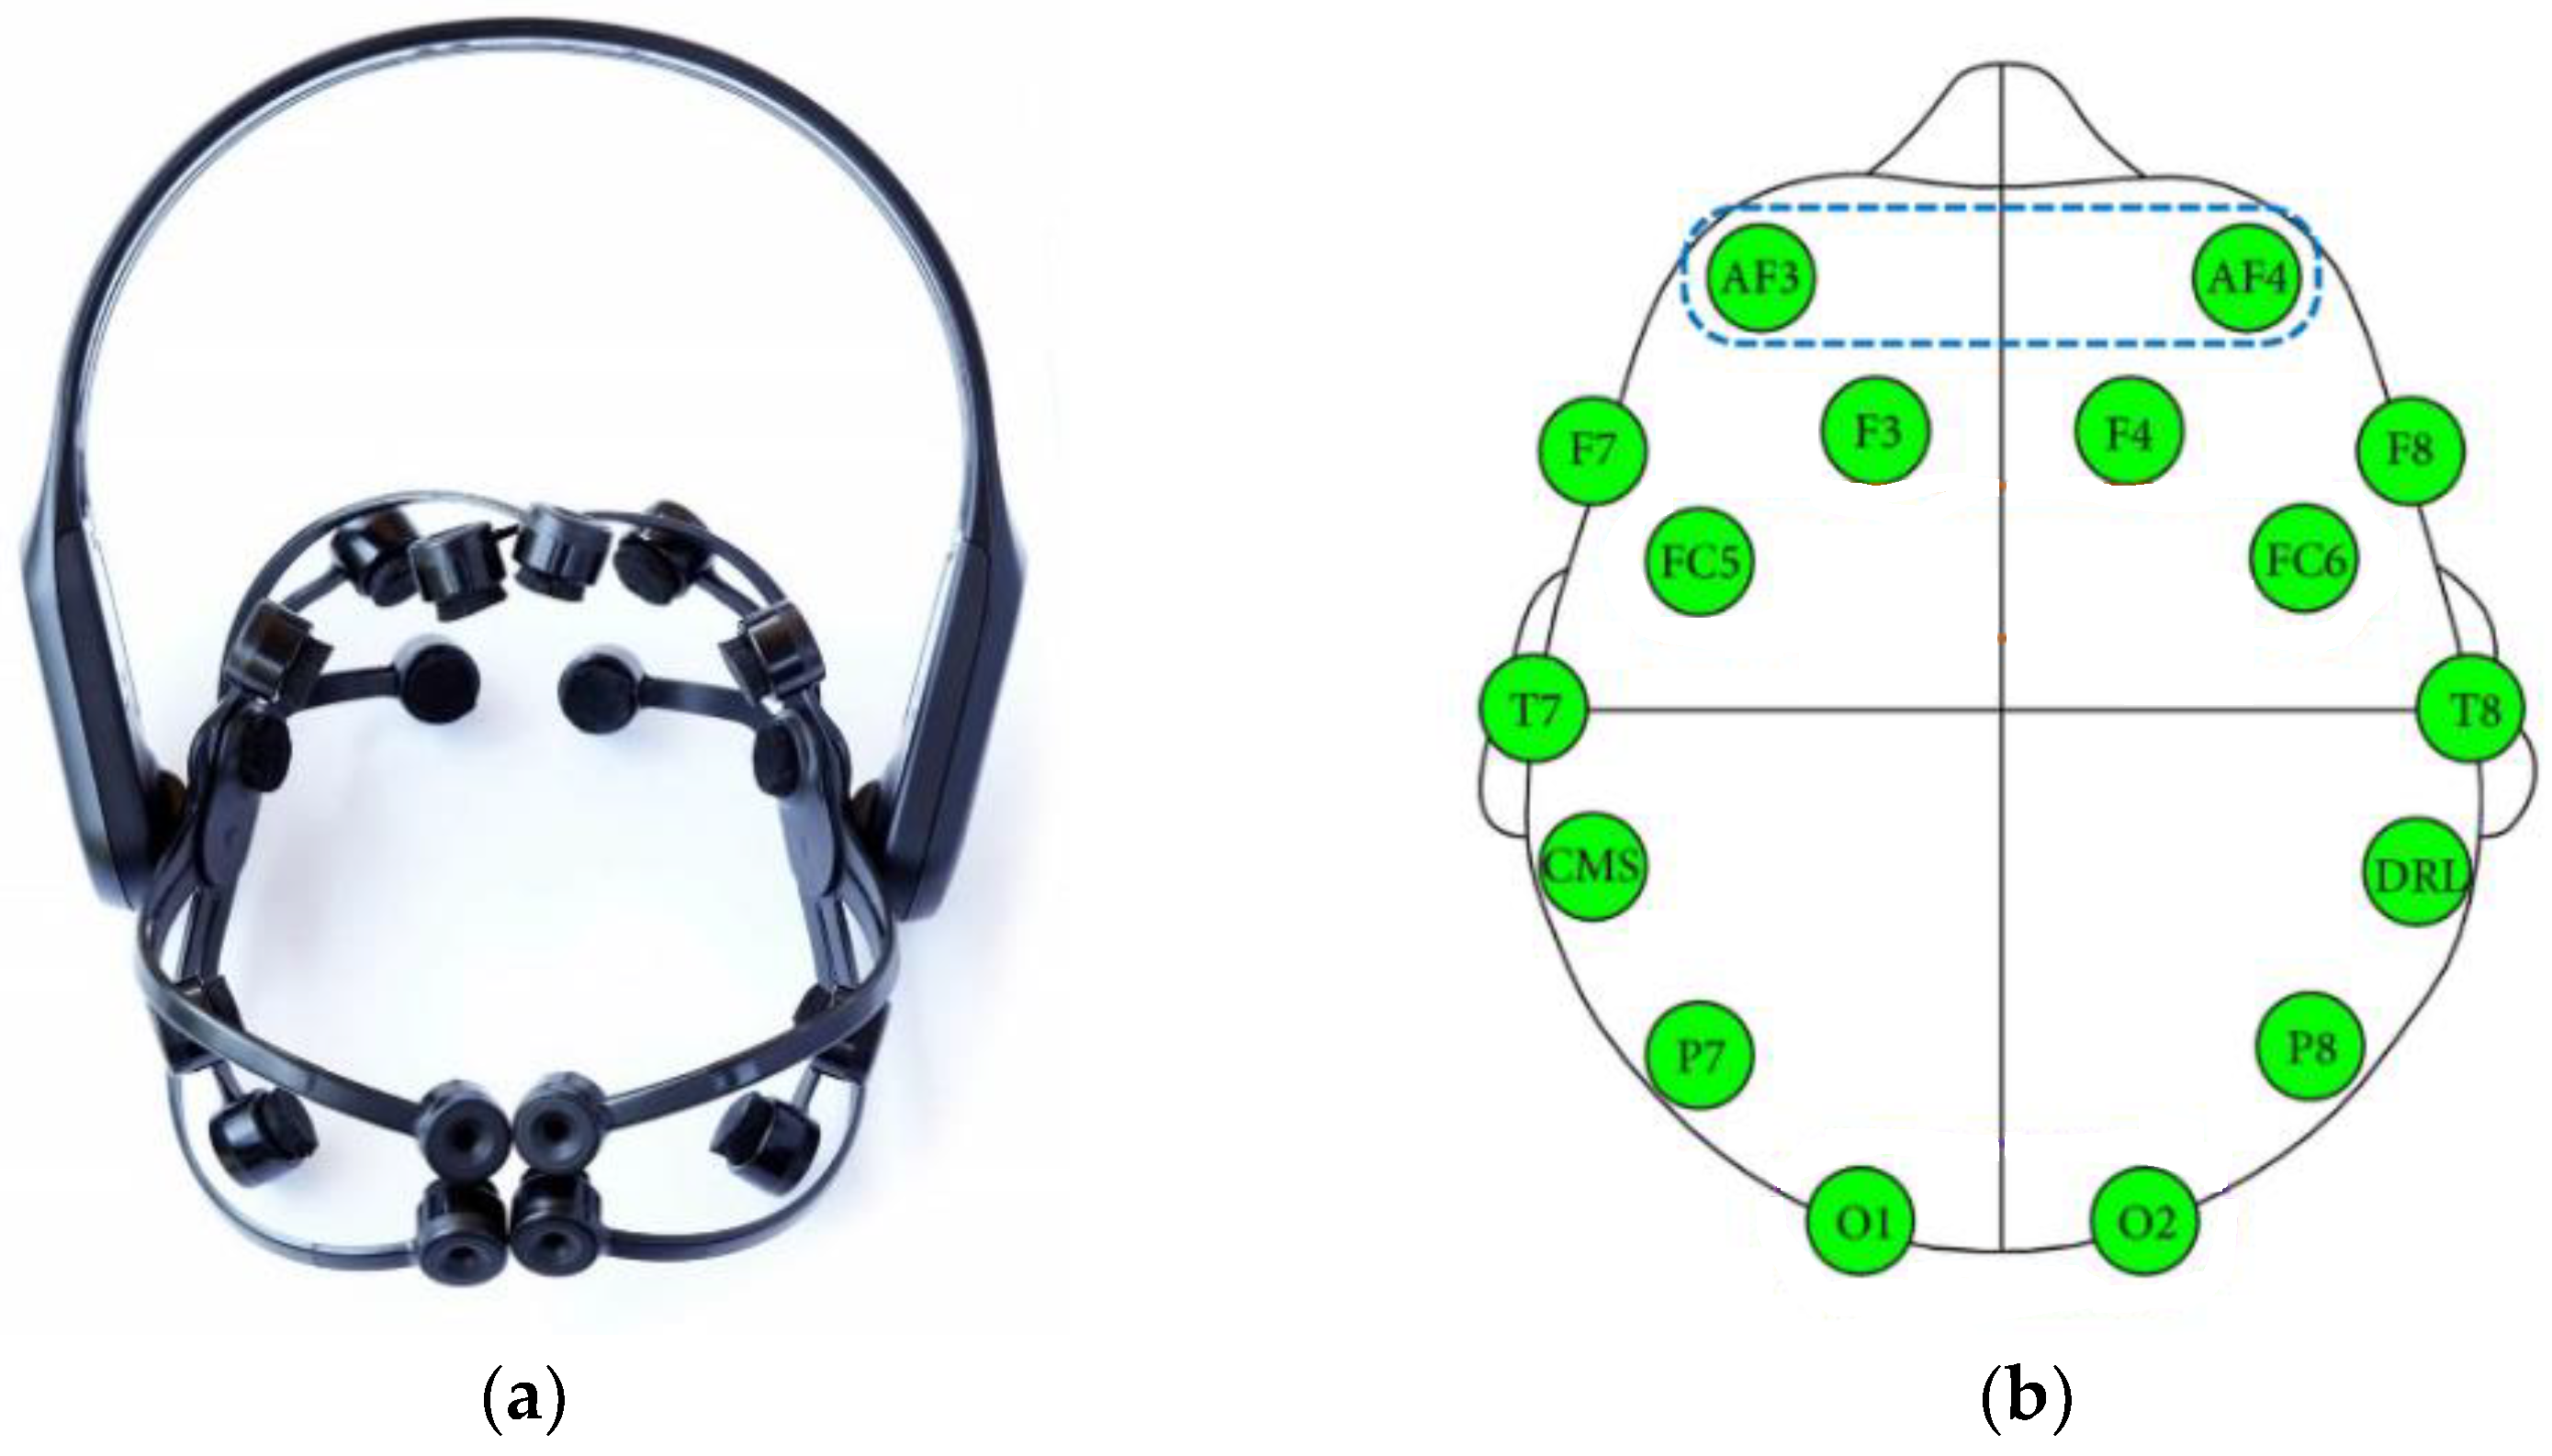
\includegraphics[width=\linewidth]{3.png}
\caption{Used the Emotiv Epoc X headset available in the lab, taking AF3and AF4 as reference electrodes, and F3 and F4 as main source for raw EEG}
\label{fig:emotiv_headset}
\end{figure}
In practical EEG acquisition systems, electrodes positioned near the eyes serve as
optimal reference channels for capturing ocular activity. As illustrated in Figure 1,
this study utilizes the Emotiv Epoc X headset, configuring electrodes AF3 and AF4-
located in the frontal region according to the international 10-20 system-as primary
EOG reference channels. Due to their proximity to the eyes, these channels are
acutely sensitive to ocular movements, displaying pronounced amplitude variations
during artifact occurrences. Concurrently, electrodes F3 and F4 are designated as
the primary sources for raw EEG data collection.

Because EOG artifacts propagate across most EEG electrodes while remaining
highly dominant in the frontal references, the structural information captured by AF3
and AF4 is instrumental in identifying the ocular contamination footprint. By
arranging the multi-channel time-series data into a matrix (where rows represent
electrodes and columns denote time samples), cross-channel correlations can be
analyzed. This study employs Singular Value Decomposition (SVD) as a robust,
subspace-based mathematical technique to isolate these highly correlated artifact
components. SVD factorizes the data matrix into orthogonal components ordered by
their energy variance. Given that EOG artifacts typically possess larger amplitudes
and stronger spatial correlations, they map onto the components associated with
the largest singular values. By systematically identifying and discarding these
dominant singular components, the signal can be reconstructed from the remaining
subspace, effectively neutralizing ocular artifacts while meticulously preserving the
underlying brain activity.

\section{SVD Technique for Signal Separation}

Singular Value Decomposition (SVD) is a fundamental mathematical tool in numerical
linear algebra, often considered a generalization of the eigenvalue-eigenvector
representation for non-square matrices. SVD factorizes a given data matrix into
orthogonal components, providing critical insights into the energy, rank, and
fundamental structure of the data. Due to these robust properties, SVD is
extensively employed in signal processing applications such as noise reduction,
source separation, and dimensionality reduction.

Consider a scenario with $P$ observed signals recorded from distinct sensors or
electrodes. Each observed signal is mathematically assumed to be a linear mixture
of several underlying source signals combined with additive noise. Let the recorded
signals be denoted by $m_i(q)$, where $i = 1, 2, \ldots, P$ represents the electrode index
and $q$ denotes the time sample index. If the recordings consist of $r$ independent
source signals $s_j(q)$, the measured signal can be modeled as a linear combination of
these sources and a noise component $n_i(q)$. This relationship is expressed as:

\[
m_i(q) = t_{i1}s_1(q) + t_{i2}s_2(q) + \cdots + t_{ir}s_r(q) + n_i(q)
\]

where $t_{ij}$ represents the weighting coefficient determining the contribution strength
of the $j^{th}$ source signal to the $i^{th}$ recorded signal.

Using matrix notation, this linear mixing model is concisely written as:

\[
M = TS + N
\]

where:

\begin{itemize}
\item $M$ is the observed signal matrix.
\item $T$ is the mixing matrix.
\item $S$ is the source signal matrix.
\item $N$ represents the additive noise matrix.
\end{itemize}

The observation matrix $M$ contains all recorded signals arranged systematically as:

\[
M = [m(1), m(2), \dots, m(q)] \in \mathbb{R}^{P \times q}
\]

where $q$ indicates the total number of time samples. Similarly, the matrices $S$ and $N$
encapsulate the source signals and noise components across the sampled time
frame, respectively.

In the specific context of this study, the observed signal matrix $M$ is constructed
using the synchronized EEG and EOG channels. The contaminated raw EEG signals
recorded from the F3 and F4 electrodes, along with the ocular reference signals
from the AF3 and AF4 electrodes, are stacked to formulate the data matrix.
Consequently, each row of this matrix corresponds to a specific spatial signal
channel, and each column corresponds to a discrete time sample.

The Singular Value Decomposition of the data matrix $M$ is defined as:

\[
M = U \Sigma V^T
\]

\begin{figure}[!h]
\centering
\fbox{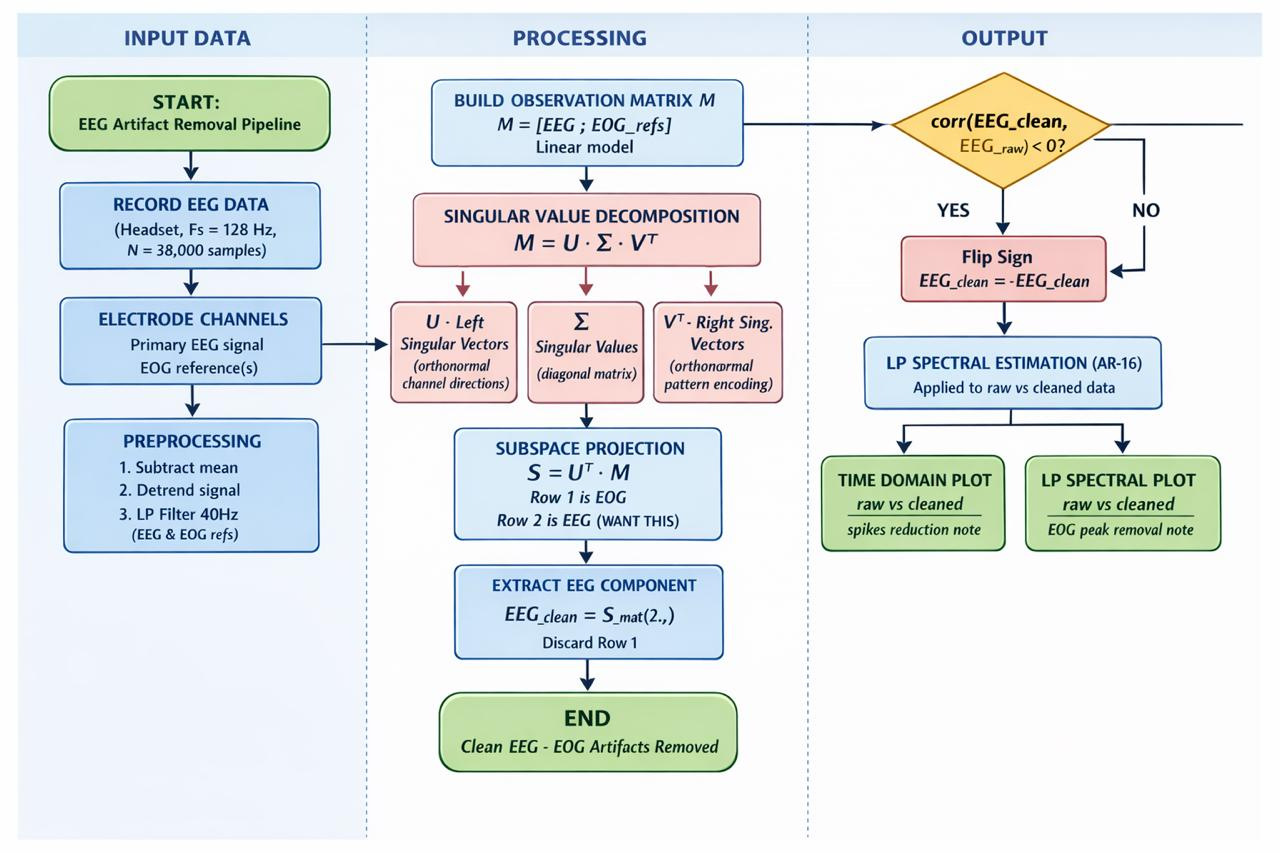
\includegraphics[width=\textwidth]{5.jpg}}
\caption{Overall workflow of the SVD-based EEG-EOG signal separation process used in this work}
\label{fig:svd_workflow}
\end{figure}

where

\begin{itemize}
\item $U$ is an orthogonal matrix whose columns are the left singular vectors, with dimensions $P \times P$.
\item $\Sigma$ is a diagonal matrix containing the singular values, with dimensions $P \times P$.
\item $V$ is an orthogonal matrix whose columns are the right singular vectors, with dimensions $P \times q$.
\end{itemize}

The diagonal elements of $\Sigma$, denoted mathematically as:

\[
\Sigma = \text{diag}(\sigma_1, \sigma_2, \dots, \sigma_P)
\]

are the singular values of the matrix $M$. These values are strictly non-negative and
are arranged in descending order of magnitude:

\[
\sigma_1 > \sigma_2 > \dots > \sigma_P > 0
\]

These singular values quantify the signal energy captured within each respective
orthogonal component. Typically, the largest singular values correspond to the
dominant, high-energy signal components, whereas the smaller singular values
represent lower-energy noise or background activity. When the artifact components
are significantly stronger than the background neural noise, the singular values can
be partitioned into two distinct groups: one delineating the principal signal subspace
and the other representing the noise subspace. Accordingly, the left singular vector
matrix $U$ can be partitioned as:

\[
U = [U_s\ U_n]
\]

where $U_s$ contains the columns spanning the signal subspace and $U_n$ contains the
columns spanning the noise subspace. Because these subspaces are orthogonal by
definition, the desired underlying signal components can be extracted by projecting
the observed multi-channel data directly onto the signal subspace. This linear
projection is computed as:

\[
S = U_s^T M
\]

The rows of this newly transformed matrix $S$ represent the decoupled principal
signal components. By strategically selecting the rows that correspond to the
desired signal subspace, the underlying neural signals can be effectively separated
from ocular noise.

As detailed in the overall workflow (Figure 2), this transformation $S = U_s^T M$ was
computationally implemented using MATLAB after performing an economy-size SVD
on the constructed data matrices. Because EOG artifacts generally possess
significantly higher amplitudes and spatial energy than standard EEG signals, the
primary dominant singular component overwhelmingly represents the ocular artifact
footprint. Therefore, the subsequent, lower-order components correspond to the
reconstructed EEG signal with drastically reduced artifact contamination. Thus, this
SVD framework provides a mathematically rigorous and highly effective
methodology for separating clean EEG signals from pervasive EOG artifacts in multi-
channel recordings.

\section{Application to Noise Reduction in EEG Signals}

The foundational step in attenuating EOG artifacts from EEG recordings involves
constructing an appropriate mathematical model for the measured data. A \textbf{linear
signal model} is predominantly employed due to its mathematical tractability and
computational efficiency. Under this paradigm, the signal recorded at each scalp
electrode is hypothesized to be a linear superposition of two primary components:
the true underlying EEG signal and a combination of EOG artifacts. Consequently,
the observed signal at the $i^{th}$ electrode is mathematically formulated as:

\[
m_i(q) = t_{i1}s_1(q) + \cdots + t_{ir}s_r(q) + n_i(q)
\]

where $m_i(q)$ denotes the measured signal, $s_j(q)$ represents the constituent EOG
artifact sources, $t_{ij}$ are the scalar mixing coefficients mapping the artifacts to the
electrodes, and $n_i(q)$ signifies the desired underlying EEG signal that we aim to
extract.

This formulation closely mirrors the general signal mixture model introduced
previously. However, a critical distinction in this specific application is the conceptual
inversion of the target components: the additive ``noise'' term $n_i(q)$ now represents
the desired true EEG data, whereas the primary source signals $s_j(q)$ act as the
ocular interference.

Leveraging the SVD framework established earlier, the observed signal matrix $M$
undergoes an orthogonal transformation defined by:

\[
S = U^T M =
\begin{bmatrix}
U_s^T M \\
U_n^T M
\end{bmatrix}
=
\begin{bmatrix}
S_s \\
S_n
\end{bmatrix}
\]

In this transformed state, $S_s$ encapsulates the components spanning the dominant
signal subspace, while $S_n$ contains the components residing in the remaining
secondary subspace. Because the underlying EEG activity is the desired signal in
this application and typically possesses lower relative energy compared to gross
EOG artifacts, the rows of $S_n$ effectively represent the reconstructed, artifact-
minimized EEG signals.

In the practical implementation of this study, the observation matrix $M$ is
synthesized by concatenating the contaminated primary EEG signal (from either the
F3 or F4 electrode) with the corresponding ocular reference signals (AF3 and AF4),
which primarily capture ocular activity. Following matrix construction, Singular Value
Decomposition is applied, and the matrix transformation $S = U^TM$ is executed
computationally within MATLAB.

Given the high-amplitude, high-energy nature of EOG artifacts, they inherently
govern the first principal singular component. The subsequent, orthogonal singular
components capture the much weaker neural fluctuations, thereby allowing the raw
EEG to correspond to these latter components with substantially reduced artifact
contamination.

Thus, by systematically selecting the appropriate lower-energy components from
the transformed matrix, the true EEG signal can be successfully reconstructed with
minimized EOG artifacts. The dimensions of the matrices and signals utilized in this
SVD-based signal model are summarized in Table 1.

\begin{table}[H]
\centering
\small
\begin{tabular}{>{\raggedright\arraybackslash}p{0.18\textwidth} >{\raggedright\arraybackslash}p{0.48\textwidth} >{\raggedright\arraybackslash}p{0.18\textwidth}}
\toprule
Symbol & Description & Dimensions \\
\midrule
$M$ & Observed signal matrix & $P \times q$ \\
$T$ & Mixing matrix & $P \times r$ \\
$S$ & Source signal matrix & $r \times q$ \\
$N$ & Noise matrix & $P \times q$ \\
$m_i(q)$ & Observed signal at electrode $i$ & $1 \times q$ \\
$s_j(q)$ & $j^{th}$ source signal & $1 \times q$ \\
$n_i(q)$ & Noise component at electrode $i$ & $1 \times q$ \\
$U$ & Left singular vector matrix & $P \times P$ \\
$\Sigma$ & Diagonal matrix of singular values & $P \times q$ \\
$V^T$ & Transpose of right singular vector matrix & $q \times q$ \\
\bottomrule
\end{tabular}
\caption{Dimensions of matrices and signals used in the SVD-based signal model.}
\end{table}

(where $P$ denotes the number of electrodes, $r$ represents the number of source
signals, and $q$ represents the number of time samples.)
\section{Results and Discussion}

\subsection{Experimental Setup and Data Acquisition}

To evaluate the empirical effectiveness of the proposed SVD-based approach for
attenuating ocular artifacts, experiments were conducted using real EEG signals
acquired from our custom dataset. The signals recorded from the frontal electrodes
F3 and F4 were designated as the primary analytical targets, while signals from the
AF3 and AF4 electrodes were utilized as reference channels capturing dominant
EOG activity.

\begin{figure}[h]
\centering

\begin{subfigure}{0.33\textwidth}
\centering
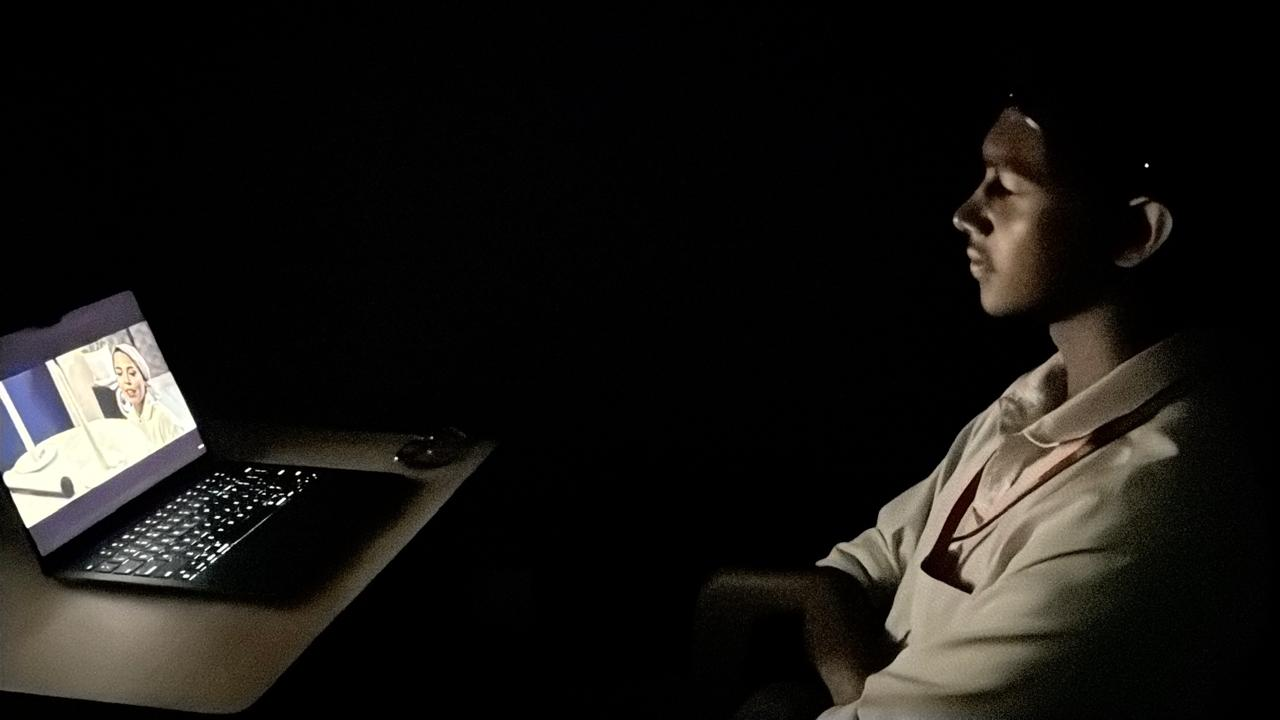
\includegraphics[width=\textwidth]{6.jpg}
\end{subfigure}
\hfill
\begin{subfigure}{0.33\textwidth}
\centering
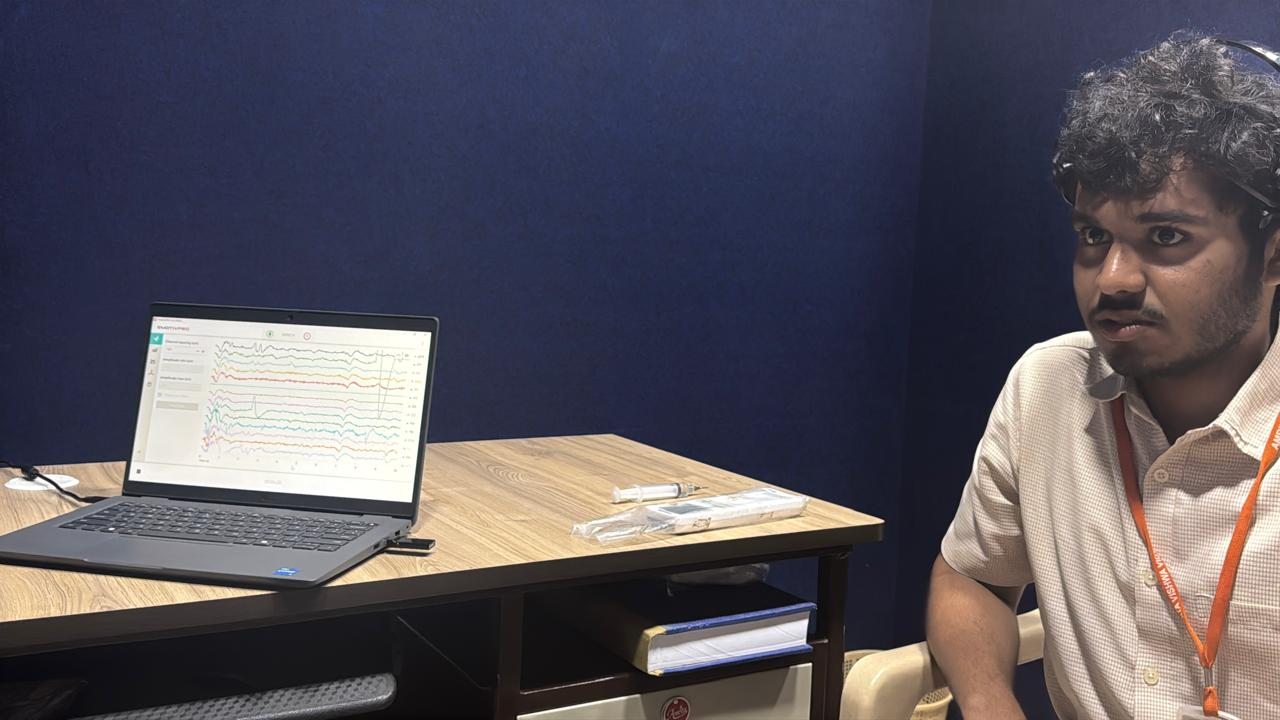
\includegraphics[width=\textwidth]{7.jpg}
\end{subfigure}
\hfill
\begin{subfigure}{0.33\textwidth}
\centering
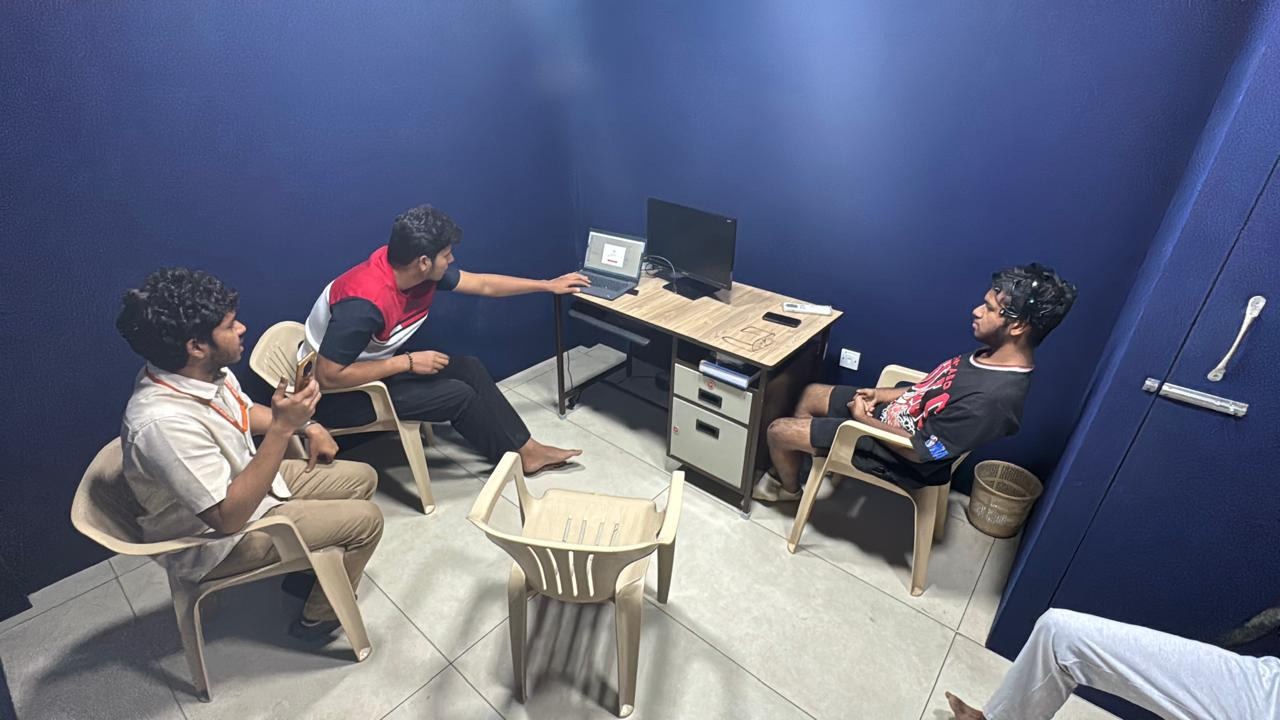
\includegraphics[width=\textwidth]{8.jpg}
\end{subfigure}
\caption{Gathering Data from the Lab}
\label{fig:lab_data_collection}
\end{figure}

Each raw EEG recording contained approximately 38,000 samples, corresponding to
300 seconds of signal duration at a sampling frequency of 128 Hz. To standardize
the evaluation, the first 60 seconds of each session were isolated for processing.
For every dataset, the contaminated primary EEG signal was concatenated with
either one (AF3) or two (AF3 and AF4) EOG reference channels to construct the
observation matrix $M$. Singular Value Decomposition was subsequently applied to
this matrix to uncouple the signal into orthogonal components.

The decomposition consistently revealed that the first singular value possessed a
significantly higher magnitude relative to the subsequent values. This mathematical
dominance confirms that the primary singular component corresponds to the EOG
artifact, as ocular movements inherently generate much larger electrical amplitudes
than underlying neural EEG signals.

\subsection{Time-Domain Signal Analysis}

The efficacy of the SVD method is immediately observable in the time-domain
morphology of the processed signals. The raw EEG signals recorded from the F3 and
F4 electrodes contain massive amplitude spikes corresponding to eye movements
and blinks. By excluding the dominant singular component and reconstructing the
signal from the remaining subspace, the artifact amplitudes are drastically
suppressed while the underlying baseline EEG activity remains structurally intact.

\begin{figure}[H]
\centering
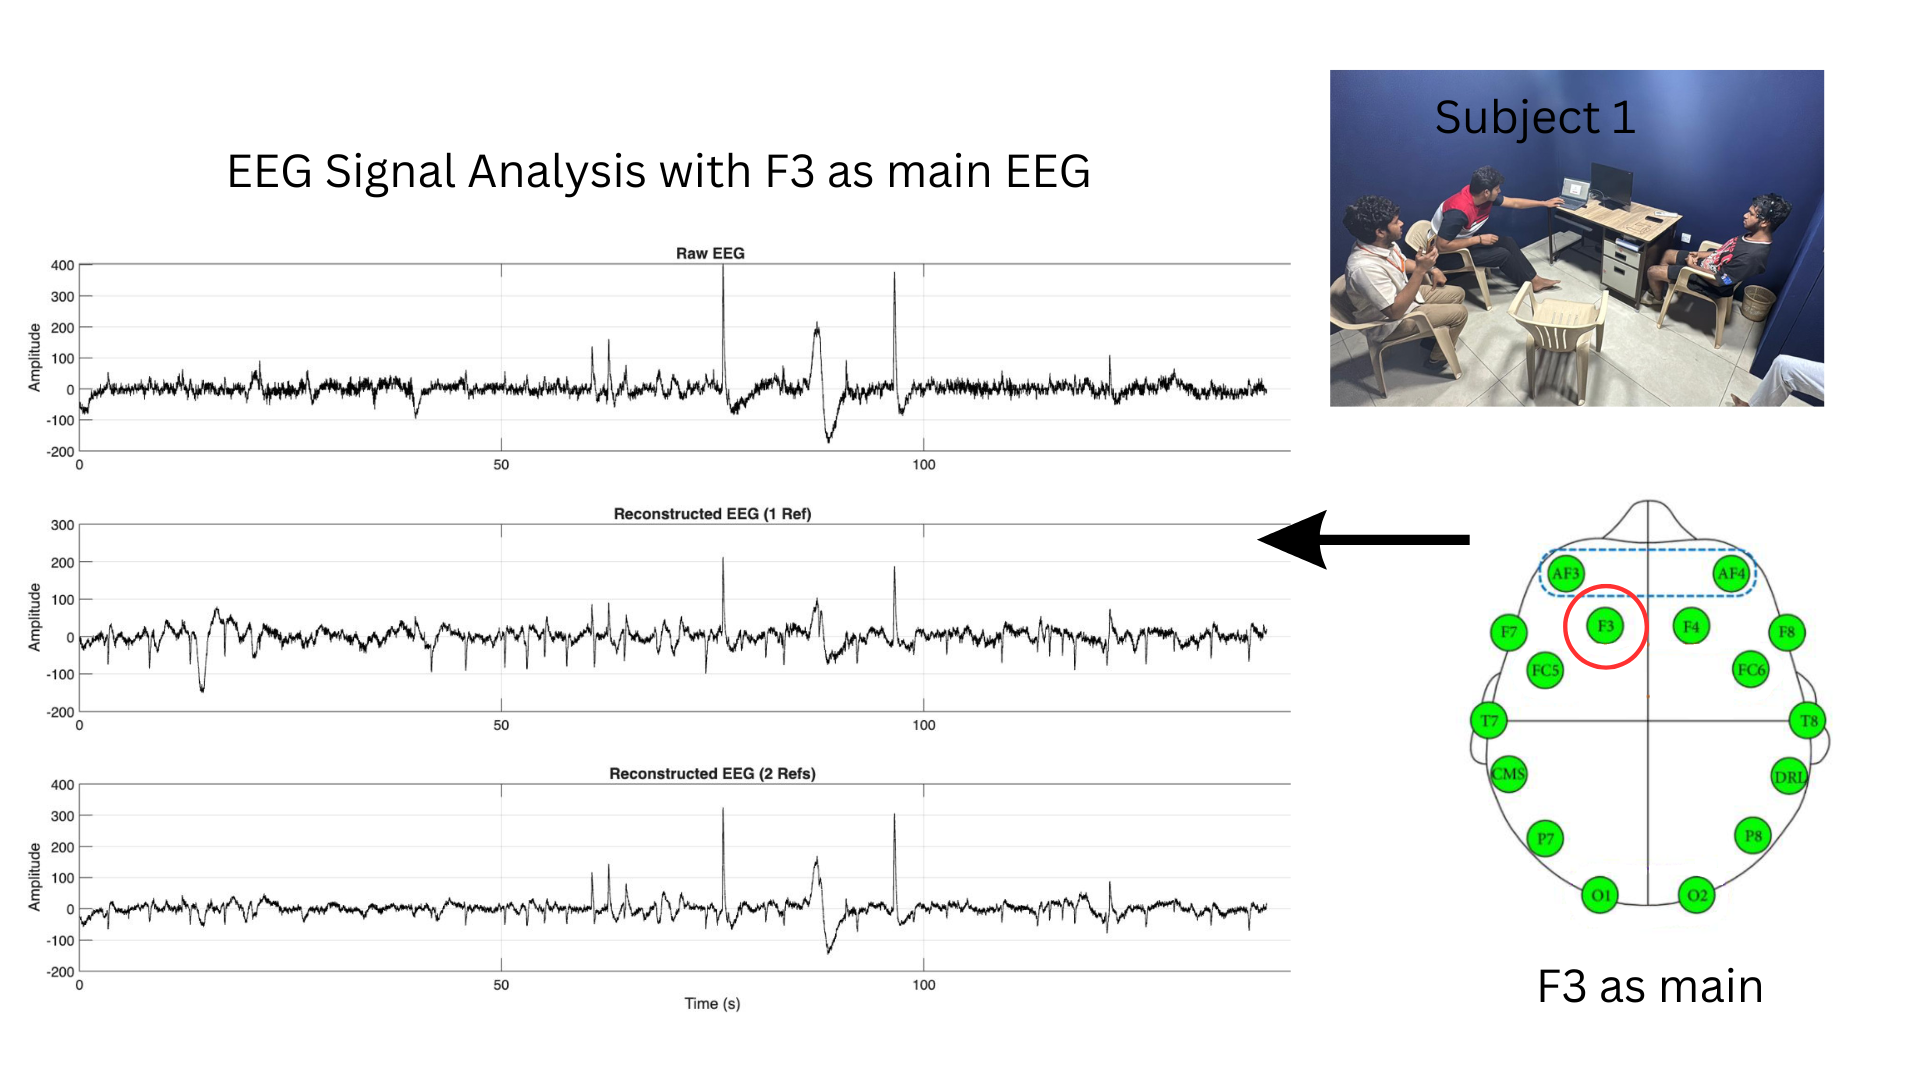
\includegraphics[width=\textwidth]{1.png}
\caption{Time-domain signals showing (a) raw EEG recorded from F3 electrode, (b) reconstructed EEG using one EOG reference channel (AF3), and (c) reconstructed EEG using two reference channels (AF3 and AF4).}
\label{fig:f3_time_domain}
\end{figure}

Figure 4 illustrates the time-domain evolution for the F3 electrode. The raw
contaminated trace exhibits severe baseline wandering and spike artifacts. Following
the SVD reconstruction using a single reference channel (AF3), the artifacts are
significantly mitigated. Incorporating the second reference channel (AF4) further
stabilizes the baseline, demonstrating superior artifact suppression.

\begin{figure}[H]
\centering
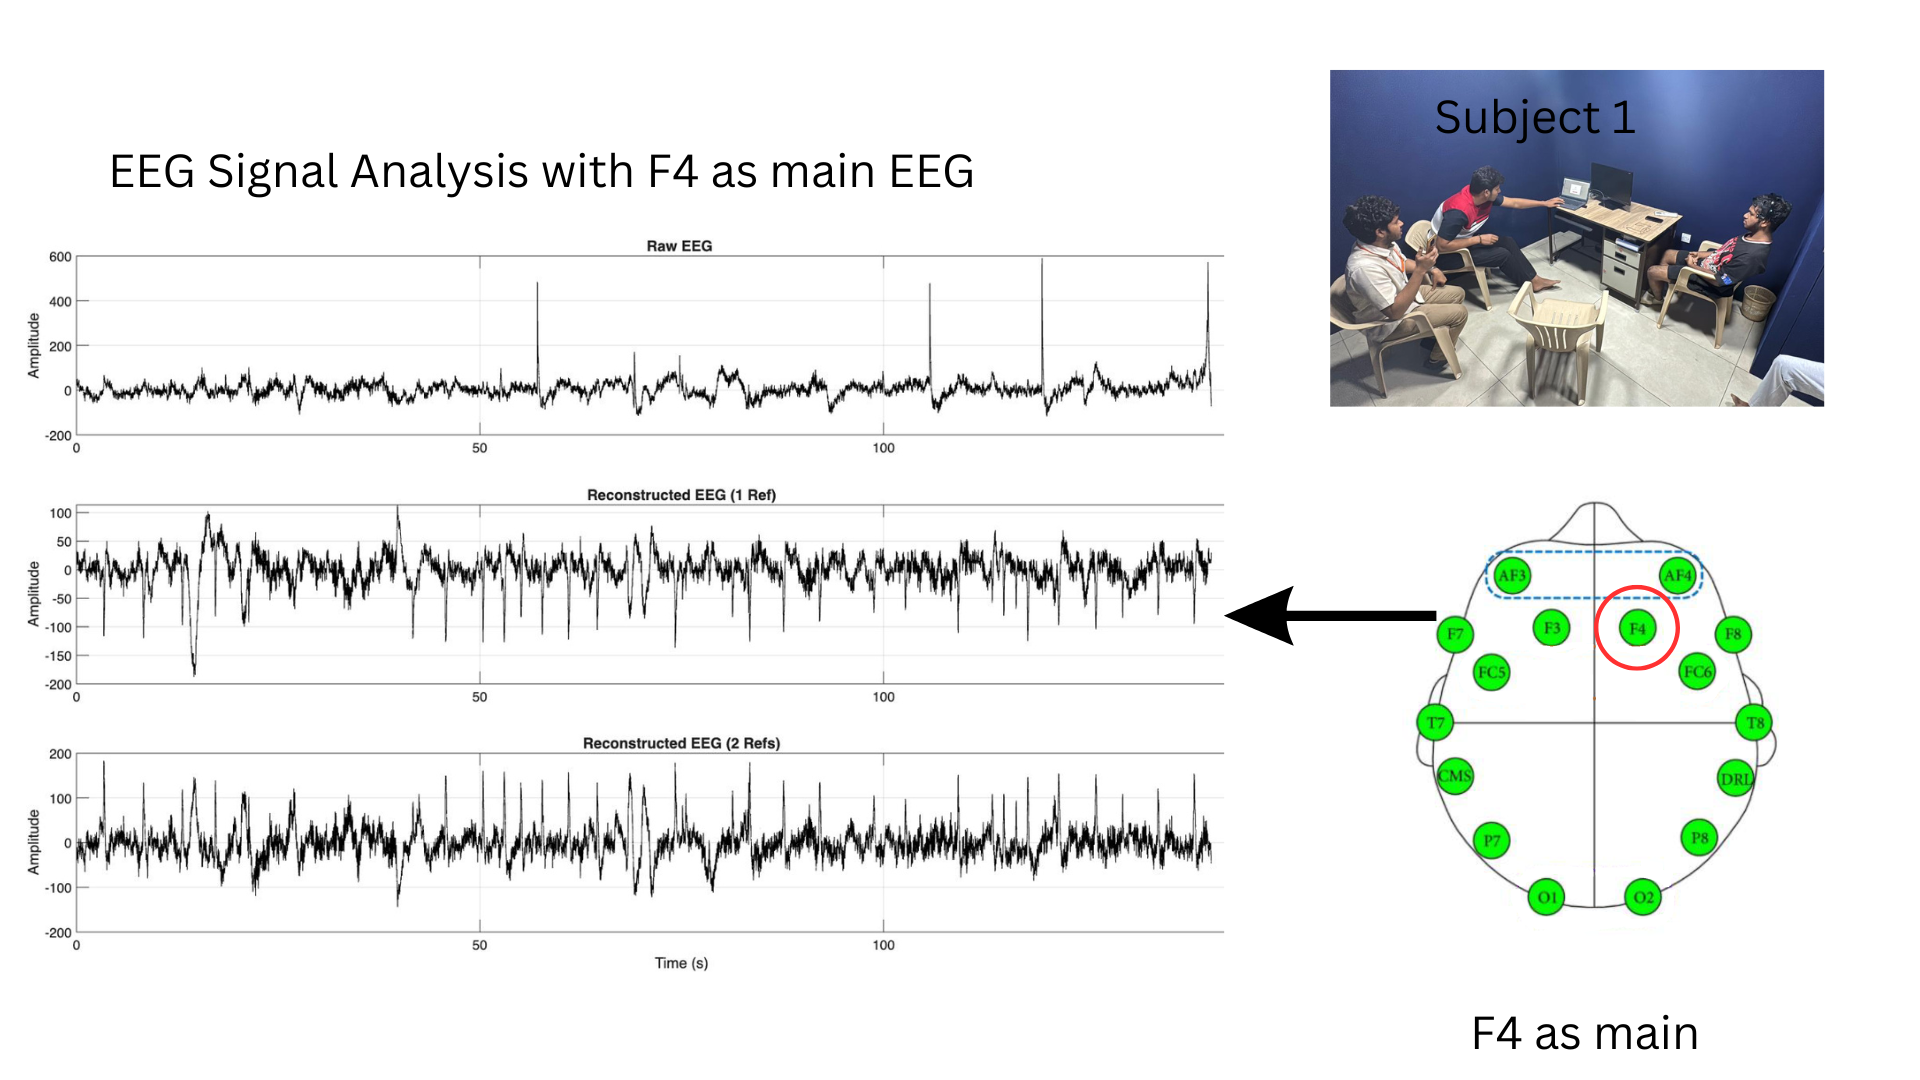
\includegraphics[width=\textwidth]{10.png}
\caption{Time-domain signals showing (a) raw EEG recorded from F4 electrode, (b) reconstructed EEG using one EOG reference channel (AF3), and (c) reconstructed EEG using two reference channels (AF3 and AF4).}
\label{fig:f4_time_domain}
\end{figure}

Because F3 and F4 are symmetric frontal electrodes within the international 10-20
system, equivalent artifact propagation patterns are expected. The parallel analysis
using the F4 electrode (Figure 6) yields nearly identical attenuation performance,
thereby validating the spatial robustness of the proposed SVD approach across the
frontal lobe.

\subsection{Spectral Analysis via Linear Prediction (LP)}

To further validate the artifact removal performance beyond temporal morphology,
the power spectrum of the signals was analyzed using Linear Prediction (LP)
spectral estimation.

\begin{figure}[H]
\centering
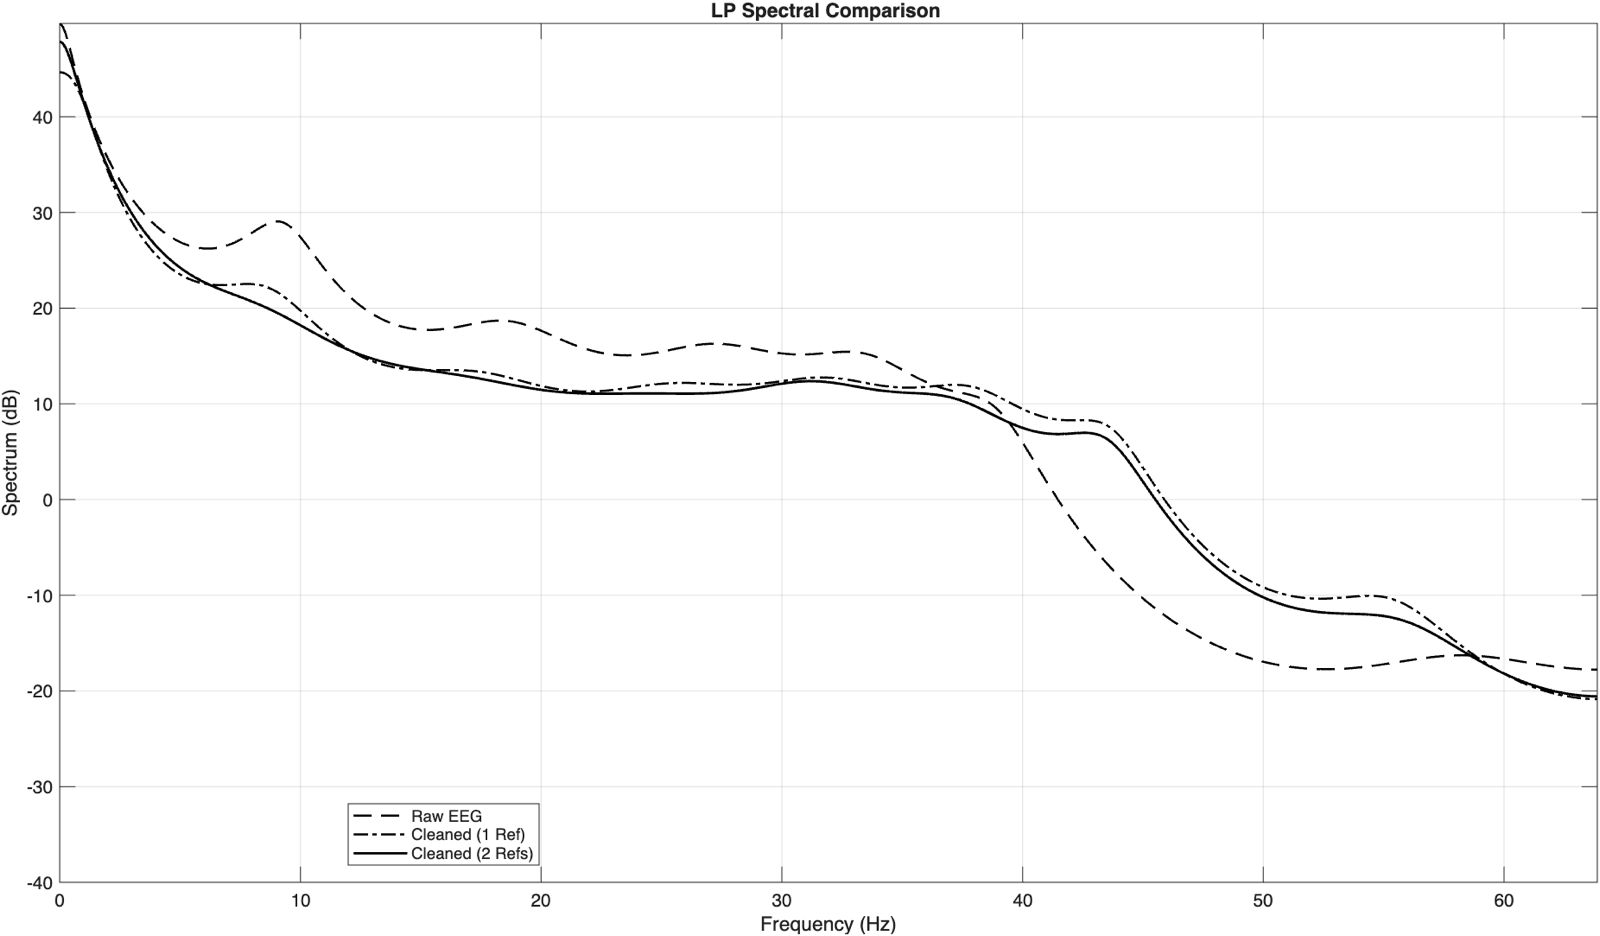
\includegraphics[width=\textwidth]{2.jpg}
\caption{Spectral comparison between raw EEG and reconstructed EEG signals obtained using one and two EOG reference channels.}
\label{fig:f3_spectral}
\end{figure}

\begin{figure}[H]
\centering
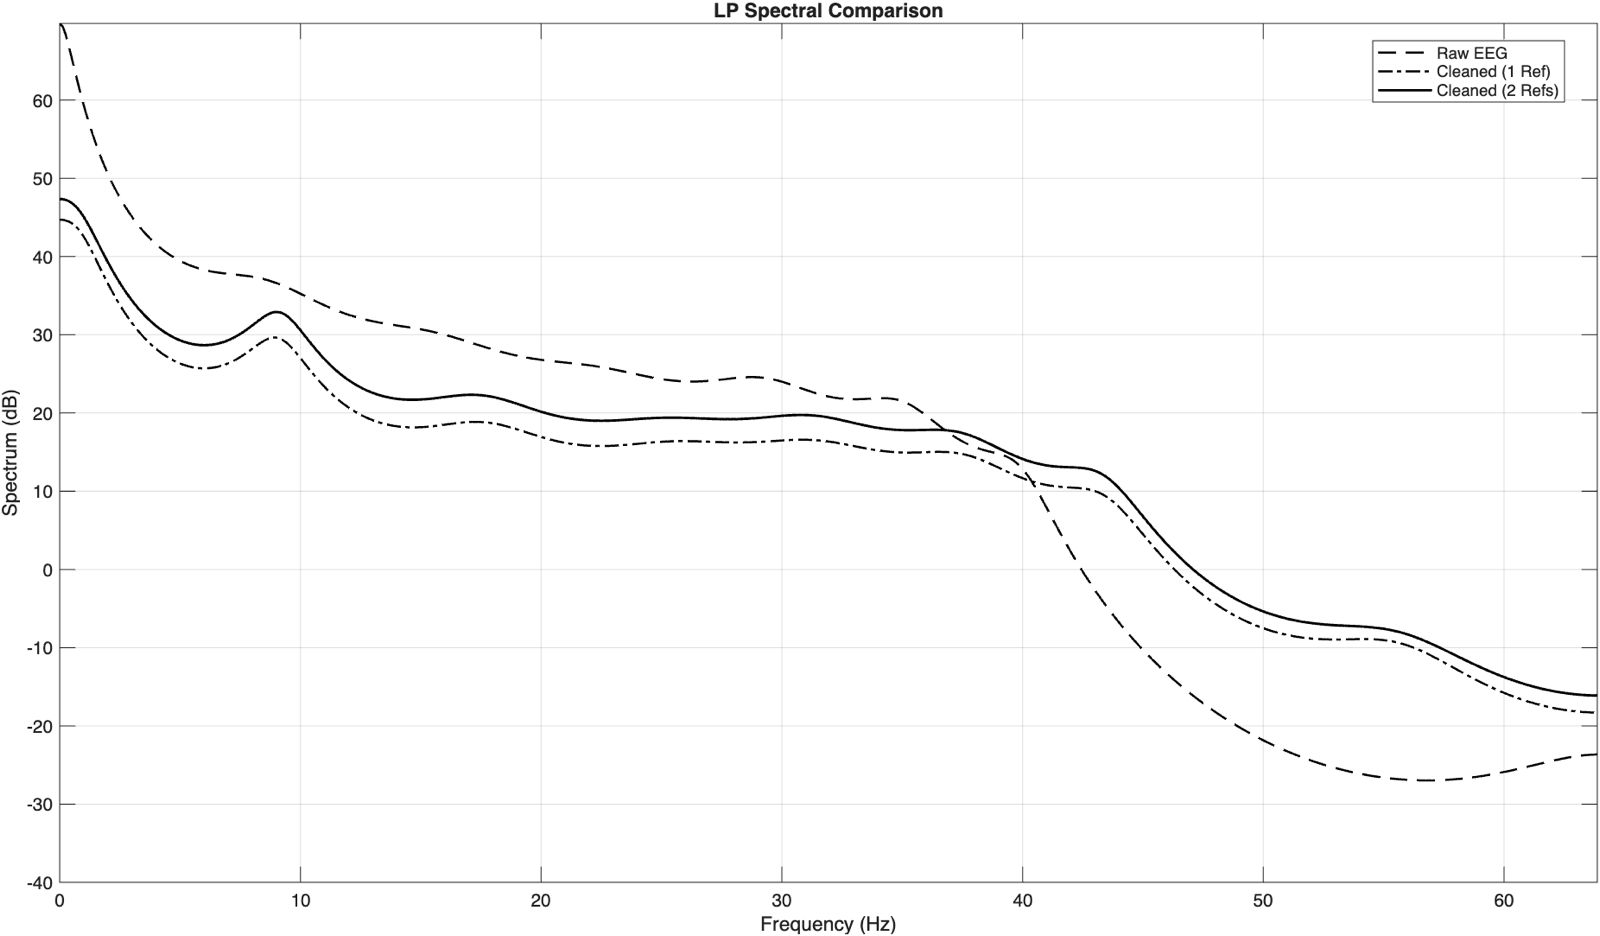
\includegraphics[width=\textwidth]{11.jpg}
\caption{Spectral comparison between raw EEG and reconstructed EEG signals obtained using one and two EOG reference channels.}
\label{fig:f4_spectral}
\end{figure}

As shown in the spectral comparison plots, the spectrum of the raw, contaminated
EEG signal exhibits an overwhelming power concentration at very low frequencies
(typically below 5 Hz), which is the hallmark signature of EOG artifacts. Following the
SVD-based subspace projection, the magnitude of this low-frequency peak is
substantially attenuated. Crucially, the spectral components at higher frequencies
(representing true neural rhythms like Alpha and Beta bands) remain largely
perfectly superimposed with the raw signal's spectrum. This spectral preservation
proves that the algorithm successfully targets and suppresses ocular artifacts
without distorting the intrinsic frequency characteristics of the brain waves.

\subsection{Quantitative Energy Analysis}

To quantify the artifact reduction, the energy loss between the original
contaminated observation matrices and the reconstructed clean matrices was
calculated using the singular values. The signal energy was derived from the
diagonal matrix $\Sigma$. Table 2 summarizes the percentage of energy removed
(representing the isolated EOG artifact energy) across six independent recording
sessions for the F3 electrode.

Table 2: Quantitative energy loss (artifact removal) across six EEG sessions (F3
Electrode)

\begin{table}[H]
\centering
\small
\begin{tabular}{>{\raggedright\arraybackslash}p{0.22\textwidth} >{\raggedright\arraybackslash}p{0.28\textwidth} >{\raggedright\arraybackslash}p{0.32\textwidth}}
\toprule
Session & Energy Loss (1 Ref: AF3) & Energy Loss (2 Refs: AF3 + AF4) \\
\midrule
Session 1 & 69.07\% & 69.14\% \\
Session 2 & 76.73\% & 88.52\% \\
Session 3 & 61.86\% & 62.73\% \\
Session 4 & 76.15\% & 82.14\% \\
Session 5 & 61.84\% & 38.47\% \\
Session 6 & 73.18\% & 86.49\% \\
\bottomrule
\end{tabular}
\end{table}

(Note: Data extracted directly from MATLAB SVD component variance calculations).

The data indicates that utilizing two EOG references generally yields a higher
percentage of energy removal, pointing to a more comprehensive isolation of
complex ocular dipole movements compared to a single reference channel.
Ultimately, by isolating the dominant artifact components from the underlying EEG
subspace, this proposed approach enables the highly reliable extraction of neural
signals from heavily contaminated recordings.

\subsection{Additional Session-wise Visualizations}

\begin{figure}[H]
\centering
\begin{subfigure}{0.495\textwidth}
\centering
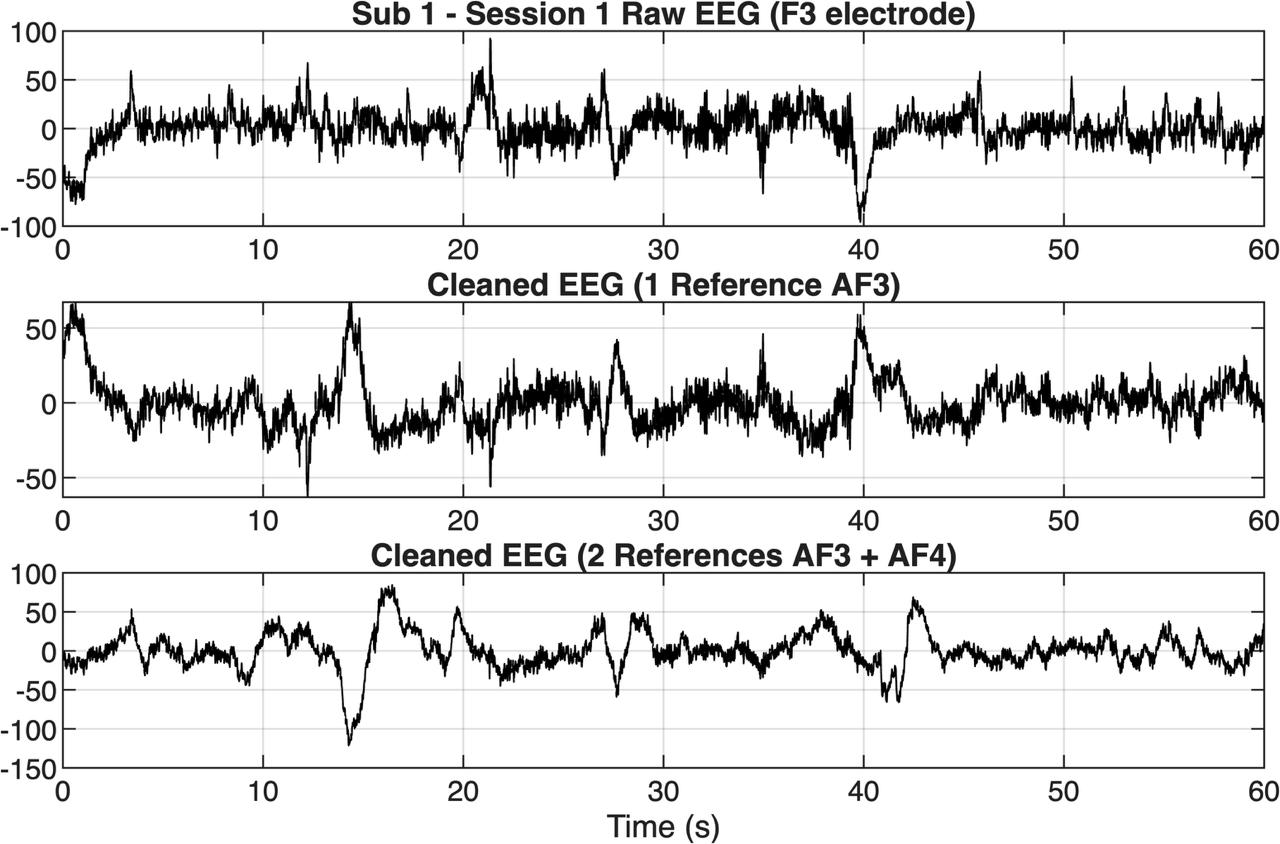
\includegraphics[width=\textwidth]{11f3.jpg}
\caption{Session 1, F3}
\end{subfigure}
\hfill
\begin{subfigure}{0.495\textwidth}
\centering
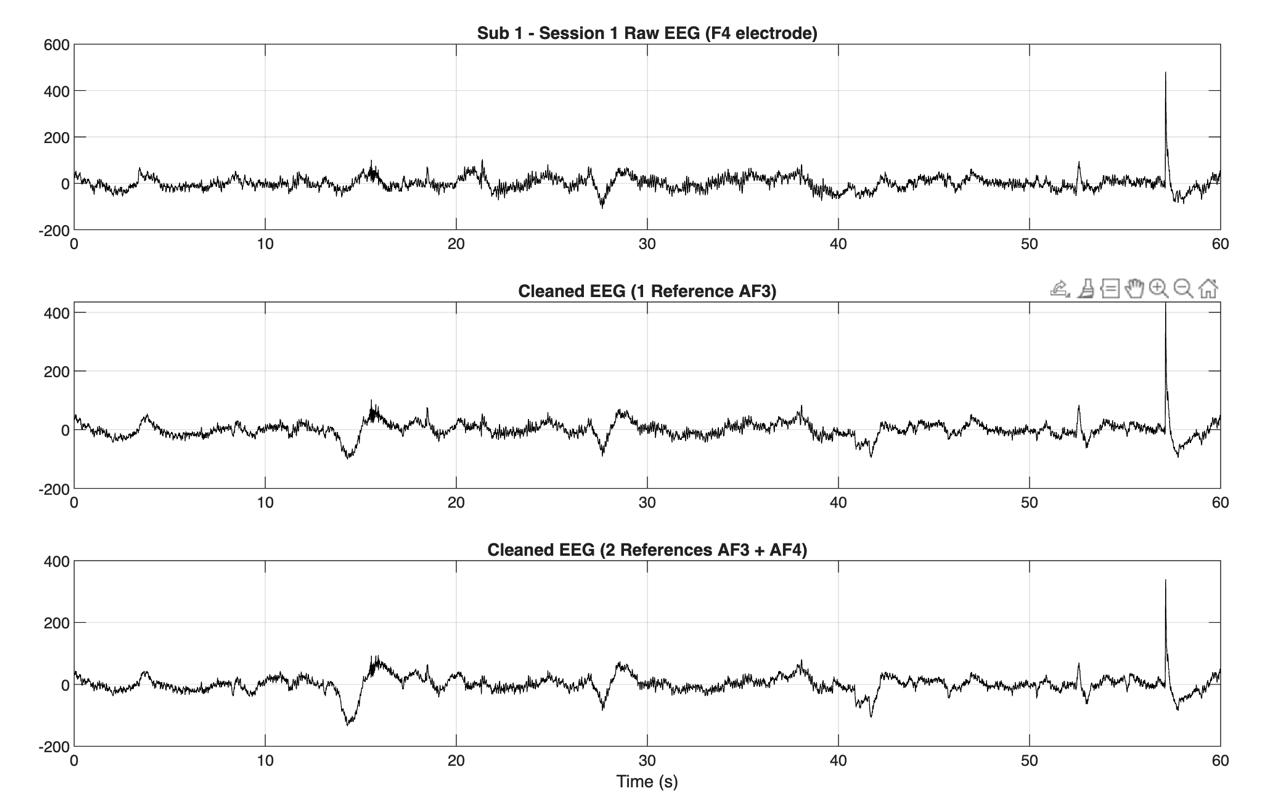
\includegraphics[width=\textwidth]{11f4.jpg}
\caption{Session 1, F4}
\end{subfigure}

\vspace{0.4cm}

\begin{subfigure}{0.495\textwidth}
\centering
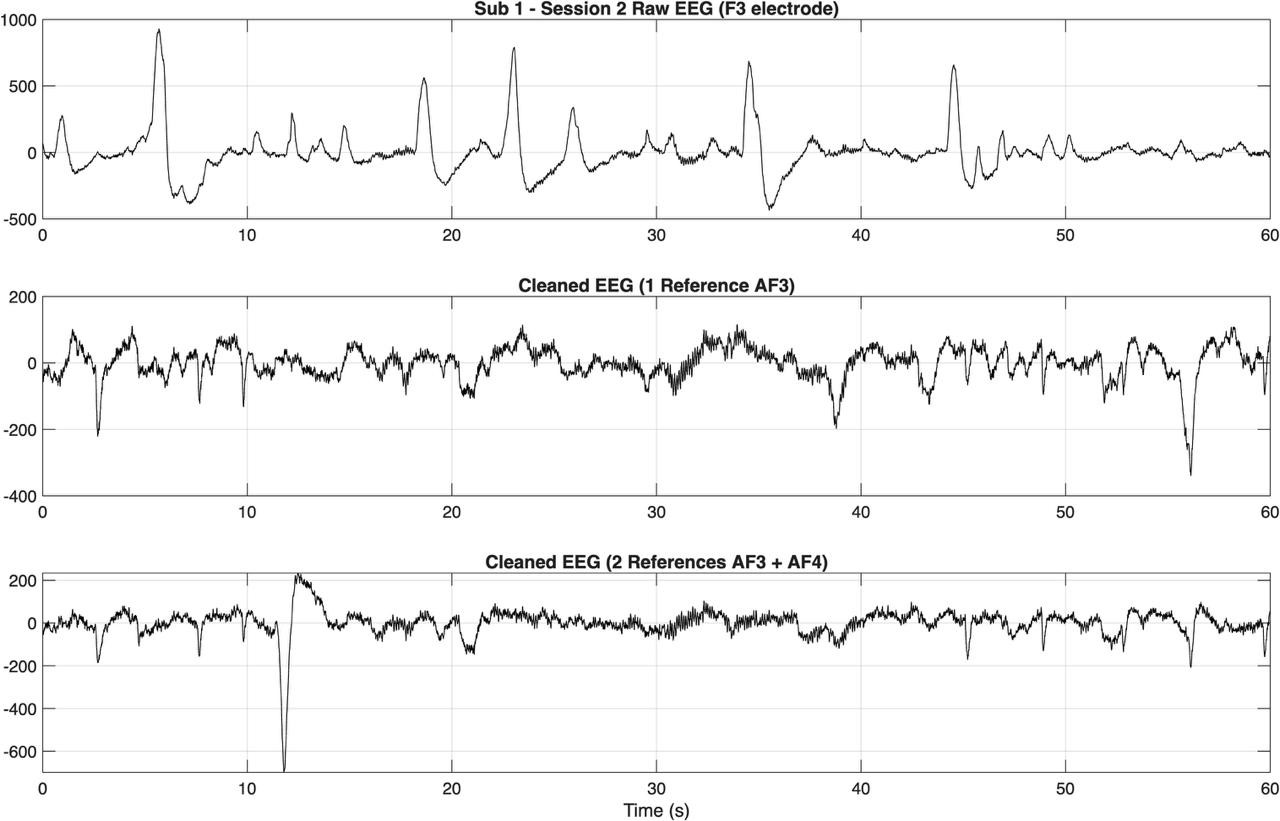
\includegraphics[width=\textwidth]{12f3.jpg}
\caption{Session 2, F3}
\end{subfigure}
\hfill
\begin{subfigure}{0.495\textwidth}
\centering
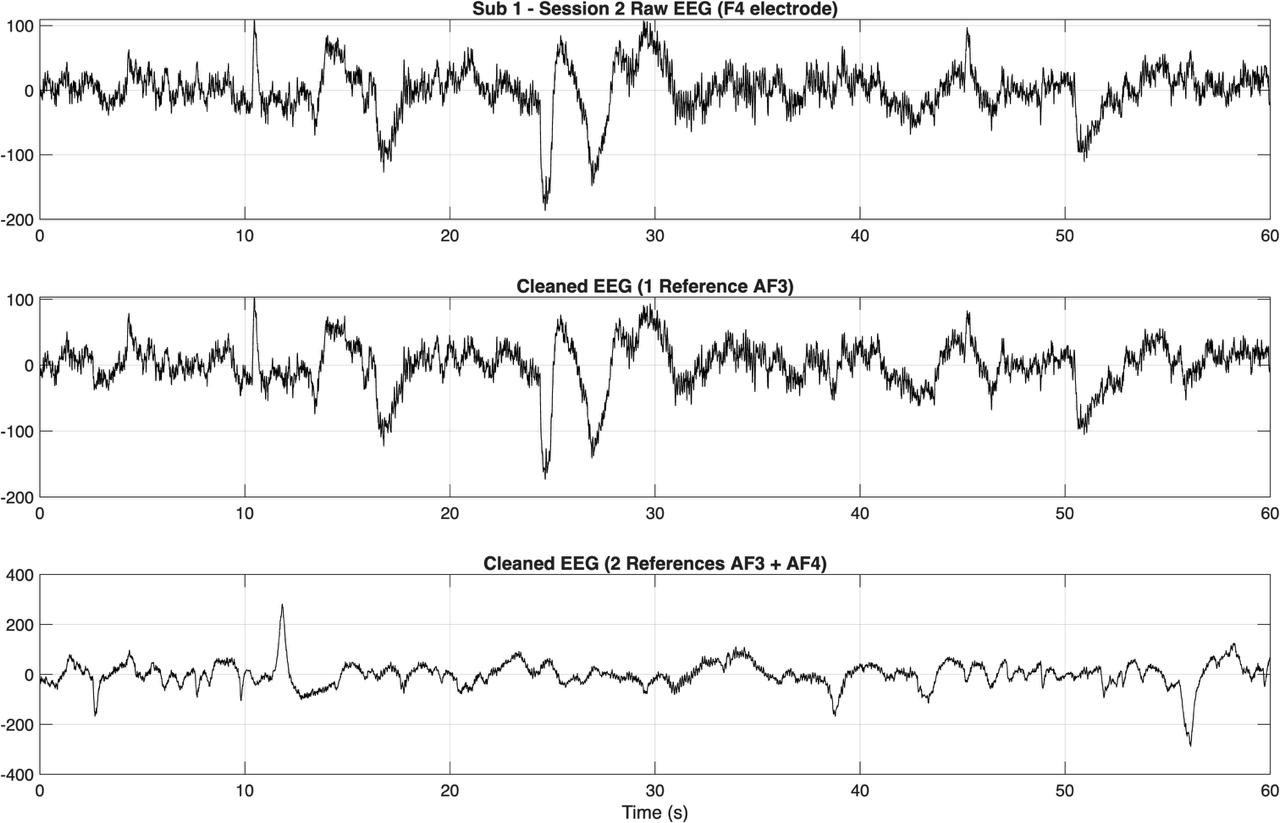
\includegraphics[width=\textwidth]{12f4.jpg}
\caption{Session 2, F4}
\end{subfigure}

\caption{Additional session-wise EEG visualizations for F3 and F4 channels.}
\label{fig:additional_sessions_11_12}
\end{figure}

\begin{figure}[H]
\centering
\begin{subfigure}{0.495\textwidth}
\centering
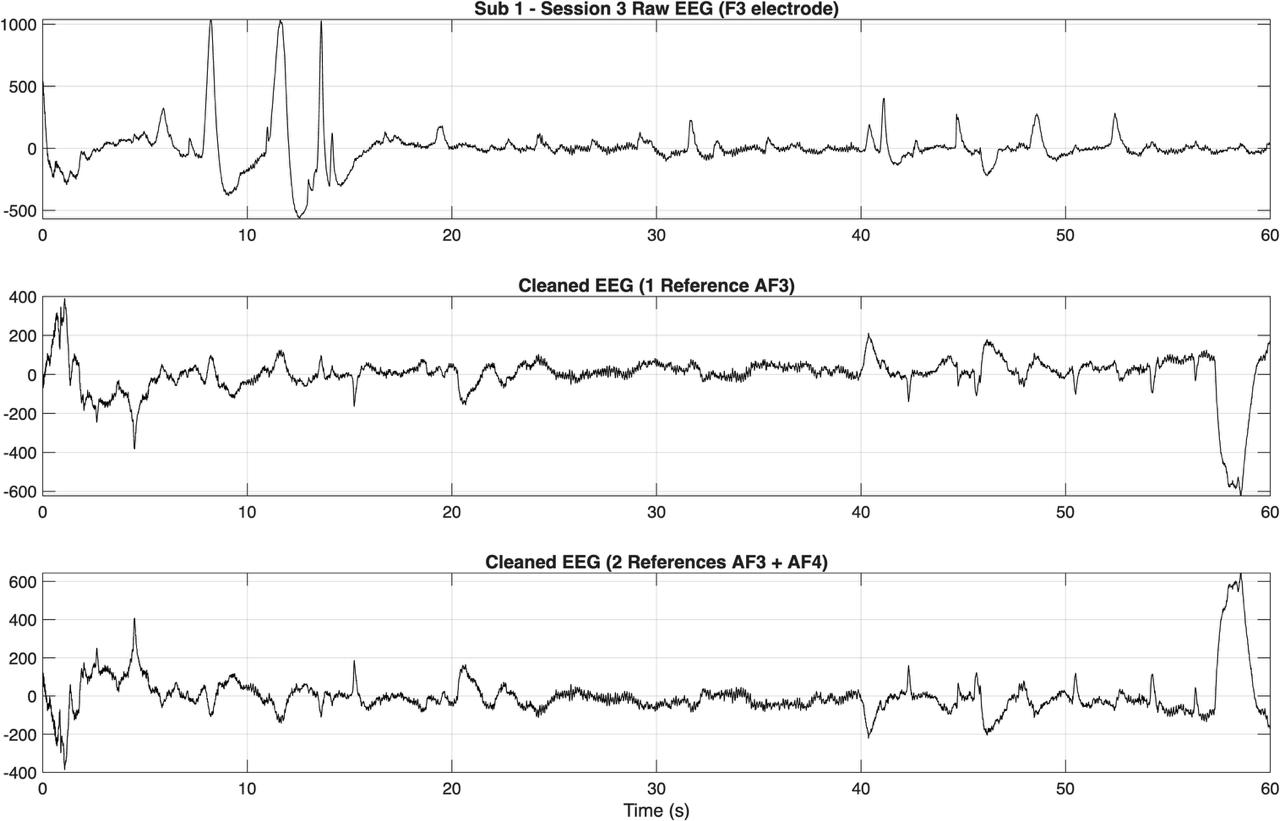
\includegraphics[width=\textwidth]{13f3.jpg}
\caption{Session 3, F3}
\end{subfigure}
\hfill
\begin{subfigure}{0.495\textwidth}
\centering
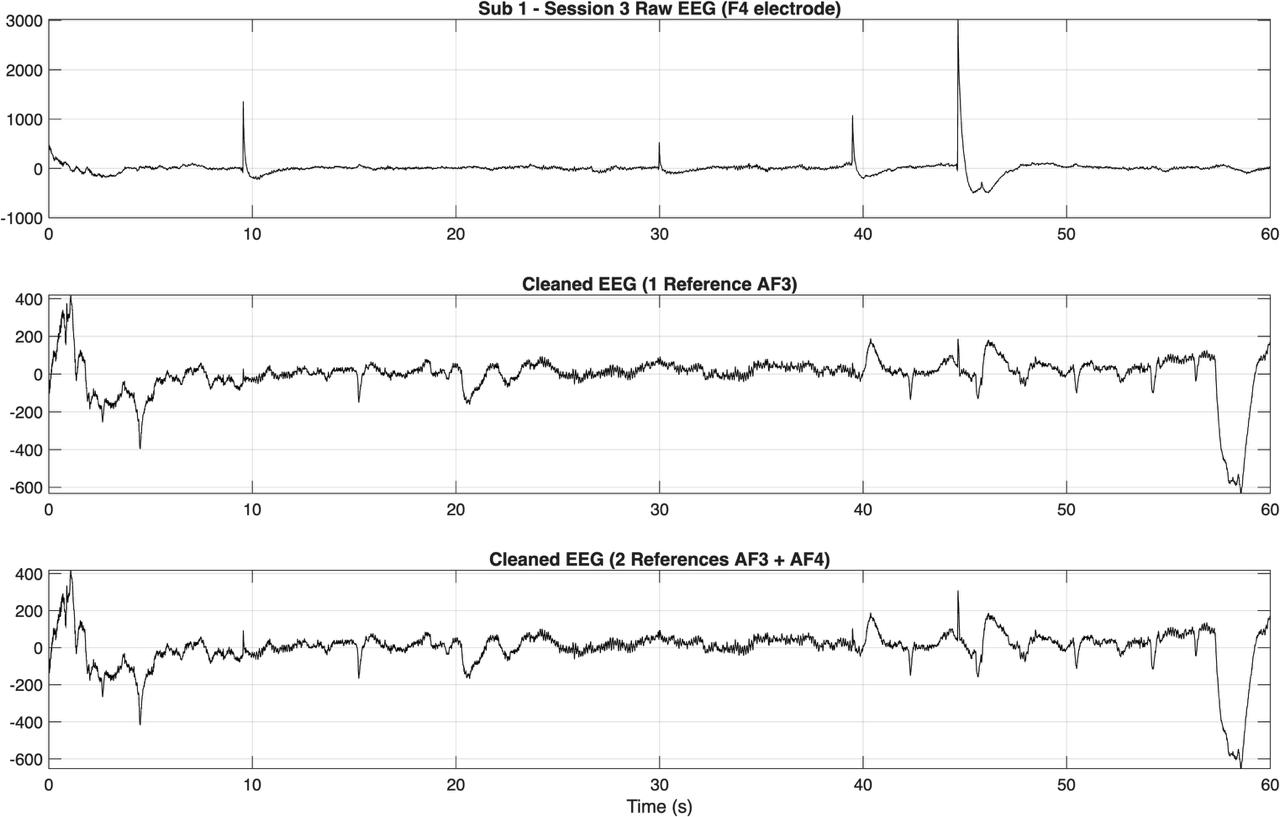
\includegraphics[width=\textwidth]{13f4.jpg}
\caption{Session 3, F4}
\end{subfigure}

\vspace{0.4cm}

\begin{subfigure}{0.495\textwidth}
\centering
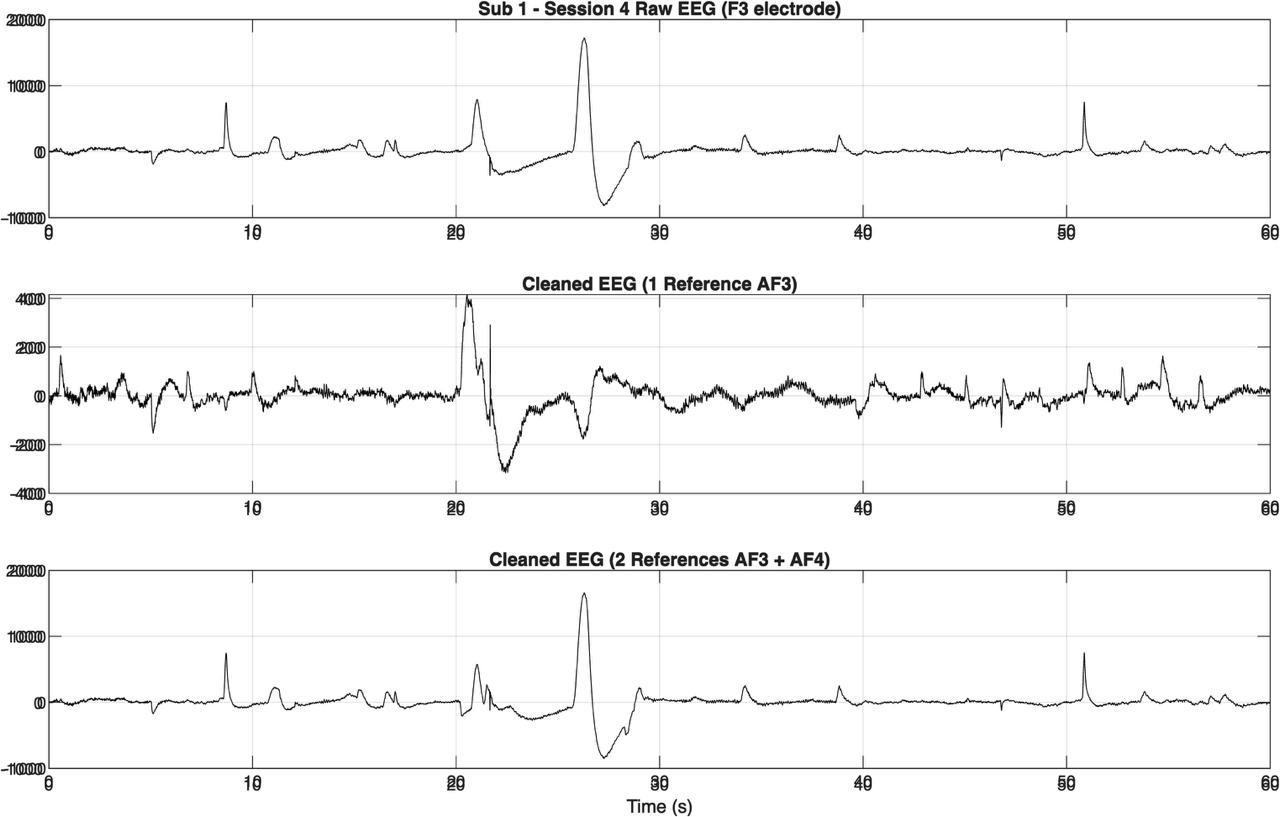
\includegraphics[width=\textwidth]{14f3.jpg}
\caption{Session 4, F3}
\end{subfigure}
\hfill
\begin{subfigure}{0.495\textwidth}
\centering
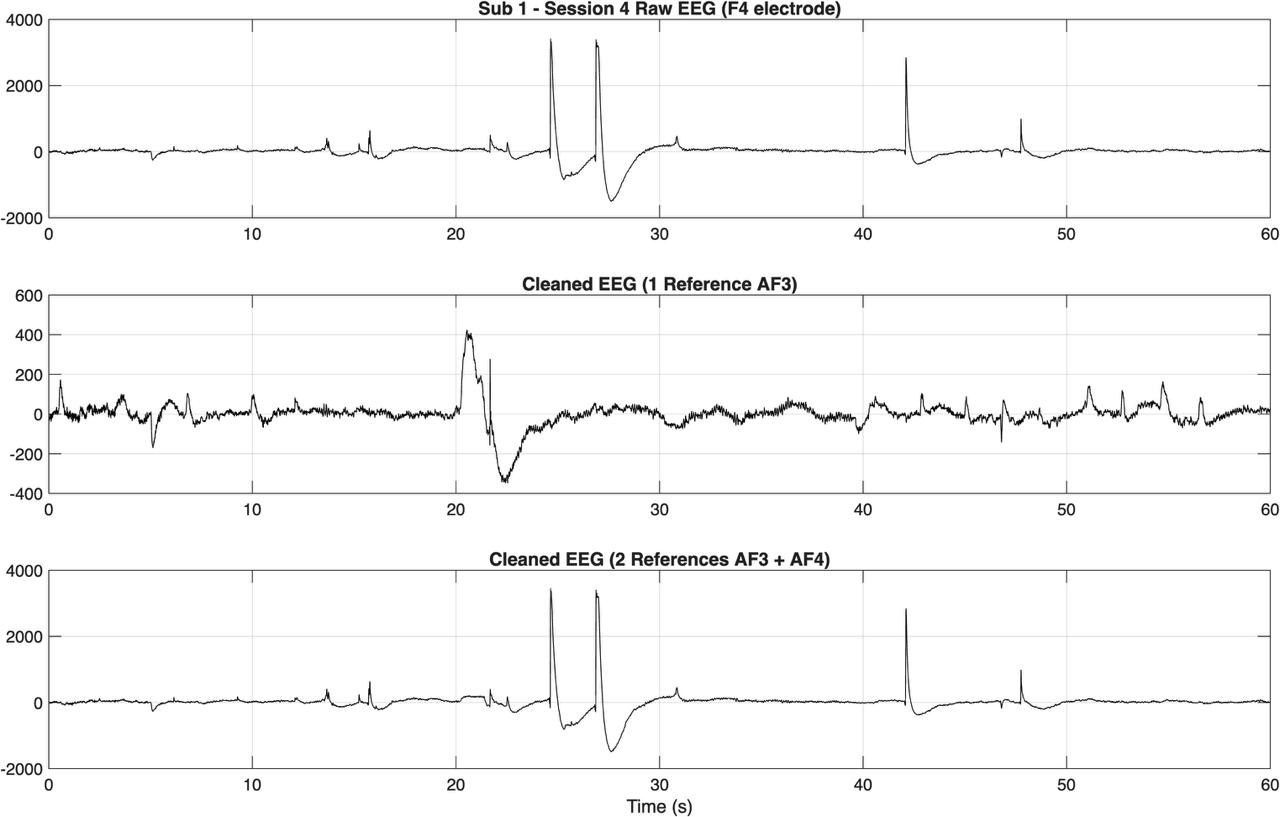
\includegraphics[width=\textwidth]{14f4.jpg}
\caption{Session 4, F4}
\end{subfigure}

\caption{Additional session-wise EEG visualizations for F3 and F4 channels.}
\label{fig:additional_sessions_13_14}
\end{figure}

\begin{figure}[H]
\centering
\begin{subfigure}{0.495\textwidth}
\centering
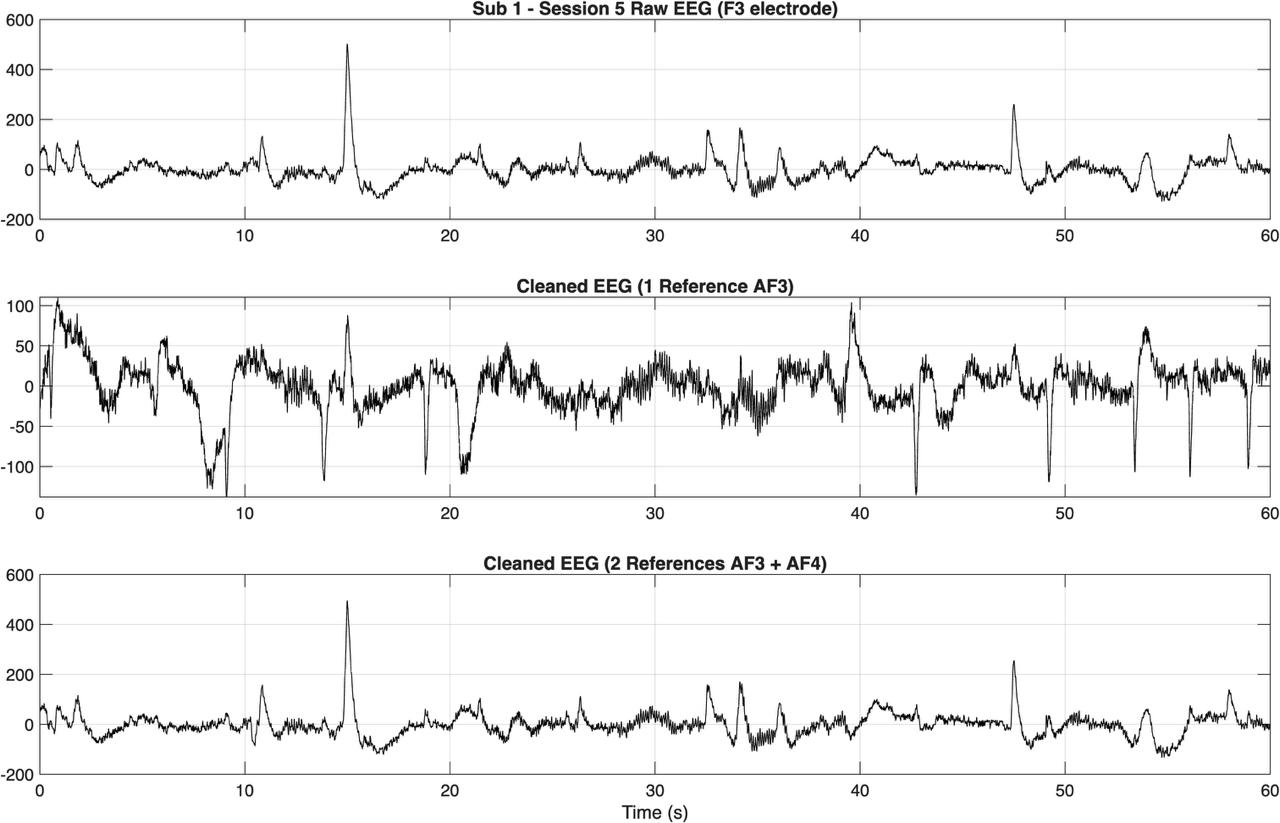
\includegraphics[width=\textwidth]{15f3.jpg}
\caption{Session 5, F3}
\end{subfigure}
\hfill
\begin{subfigure}{0.495\textwidth}
\centering
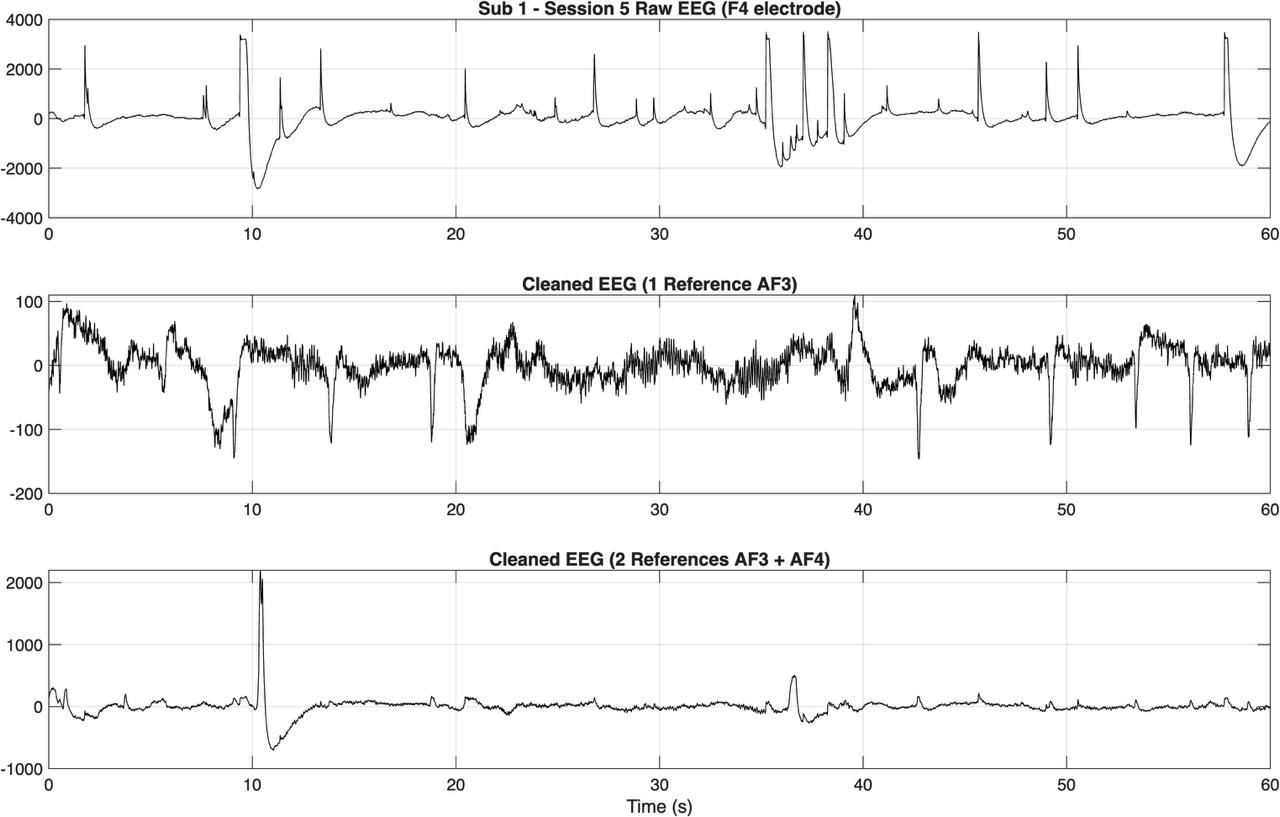
\includegraphics[width=\textwidth]{15f4.jpg}
\caption{Session 5, F4}
\end{subfigure}

\vspace{0.4cm}

\begin{subfigure}{0.495\textwidth}
\centering
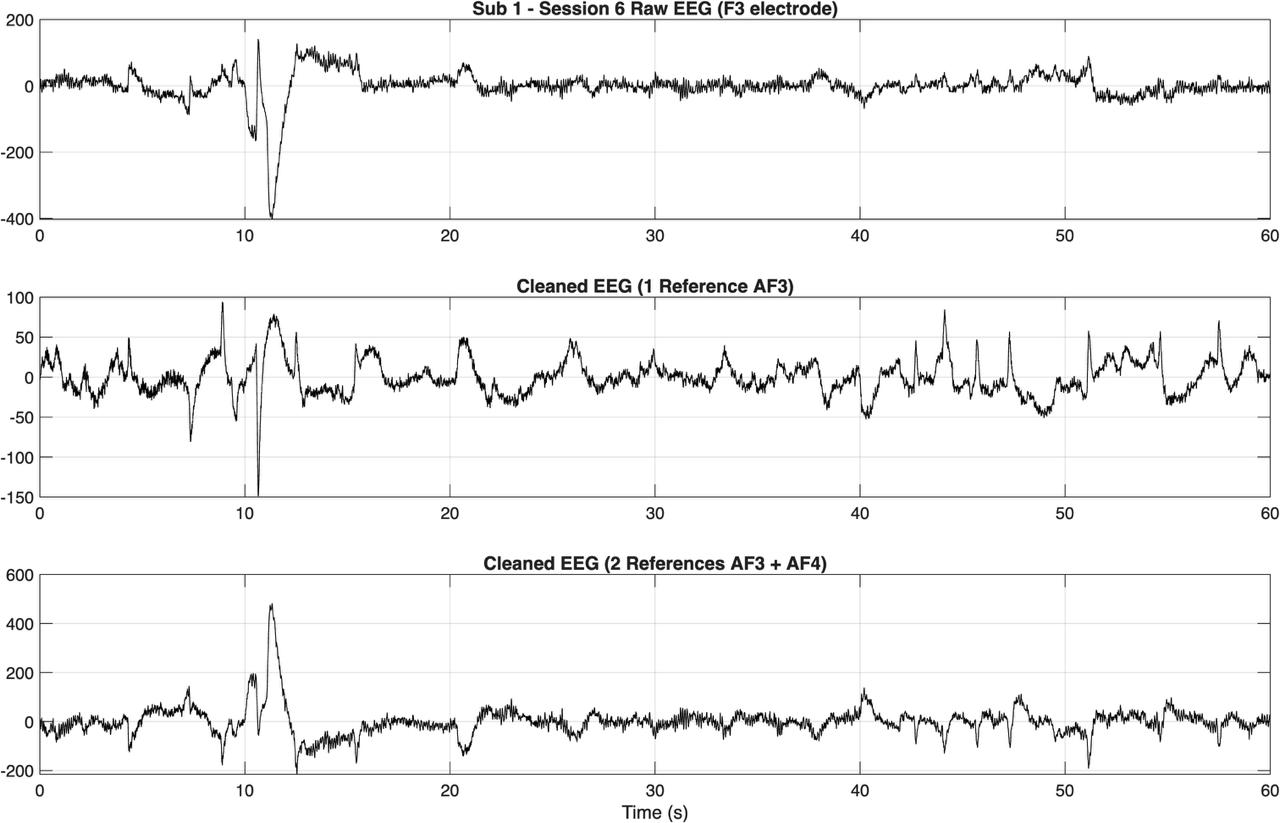
\includegraphics[width=\textwidth]{16f3.jpg}
\caption{Session 6, F3}
\end{subfigure}
\hfill
\begin{subfigure}{0.495\textwidth}
\centering
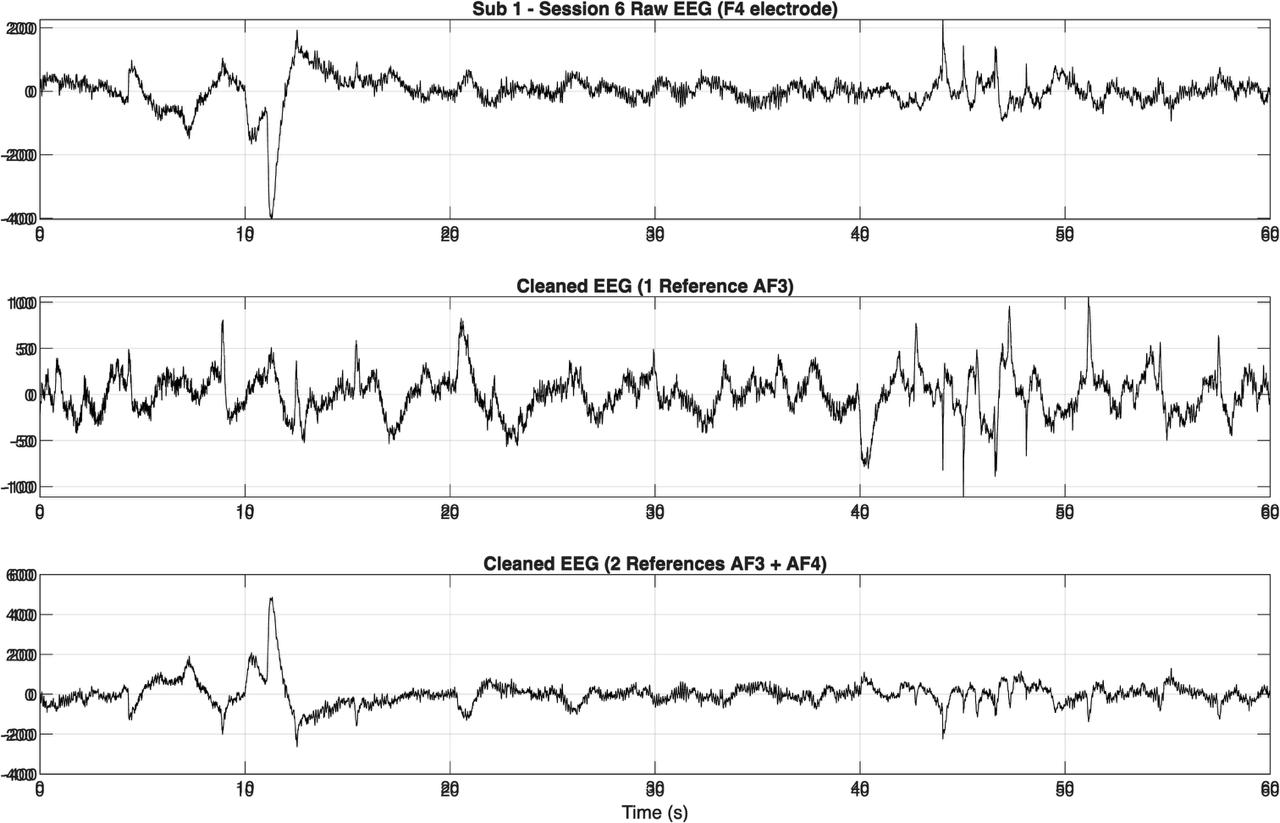
\includegraphics[width=\textwidth]{16f4.jpg}
\caption{Session 6, F4}
\end{subfigure}

\caption{Additional session-wise EEG visualizations for F3 and F4 channels.}
\label{fig:additional_sessions_15_16}
\end{figure}

\begin{figure}[H]
\centering
\begin{subfigure}{0.495\textwidth}
\centering
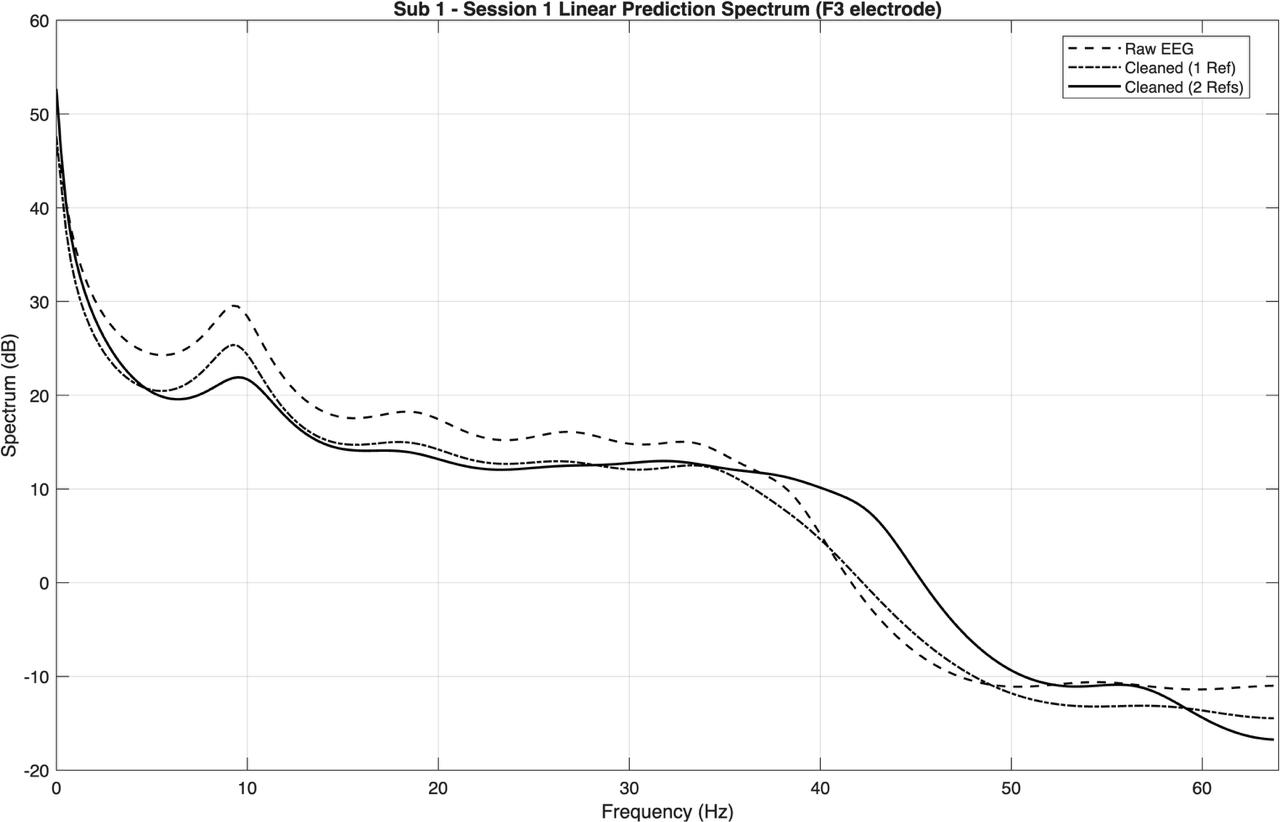
\includegraphics[width=\textwidth]{lp1f3.jpg}
\caption{LP Spectrum Session 1 (F3)}
\end{subfigure}
\hfill
\begin{subfigure}{0.495\textwidth}
\centering
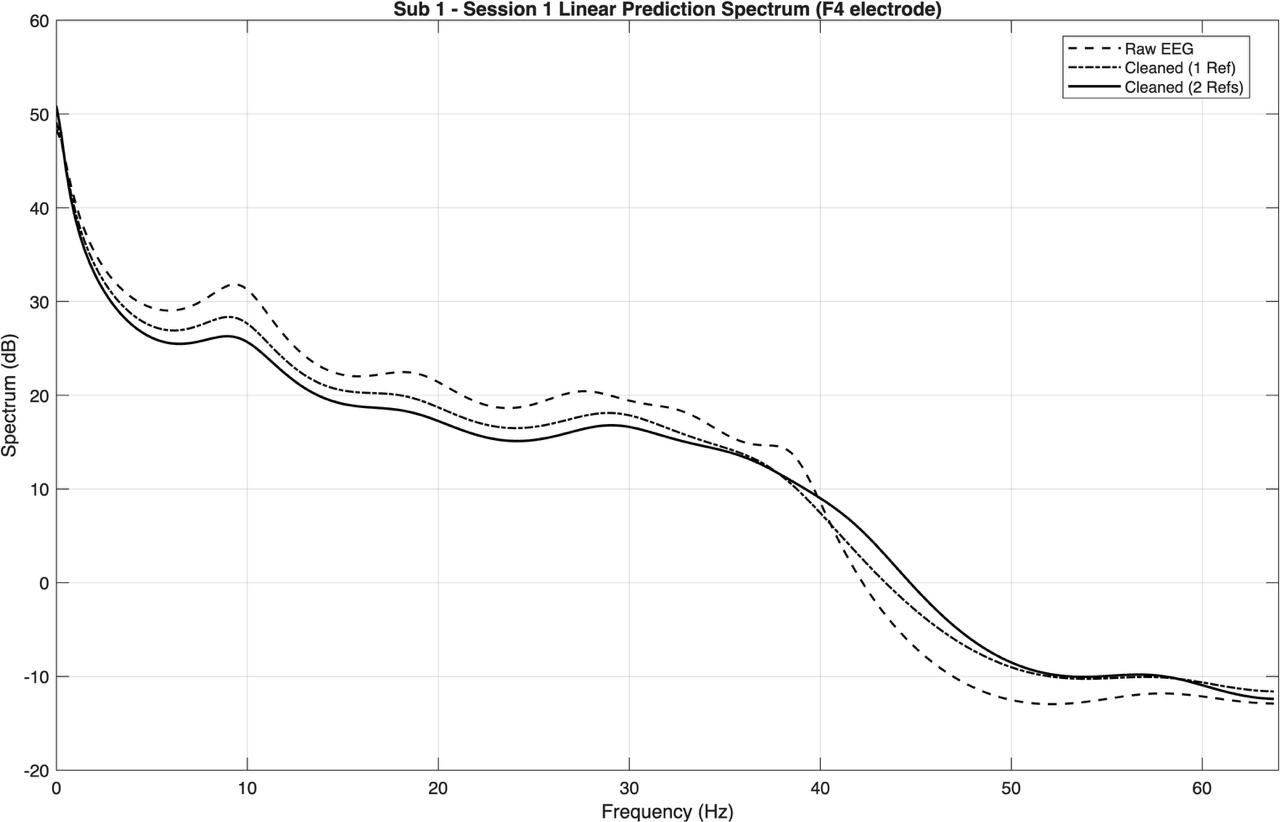
\includegraphics[width=\textwidth]{lpf4.jpg}
\caption{LP Spectrum Session 1 (F4)}
\end{subfigure}

\vspace{0.4cm}

\begin{subfigure}{0.495\textwidth}
\centering
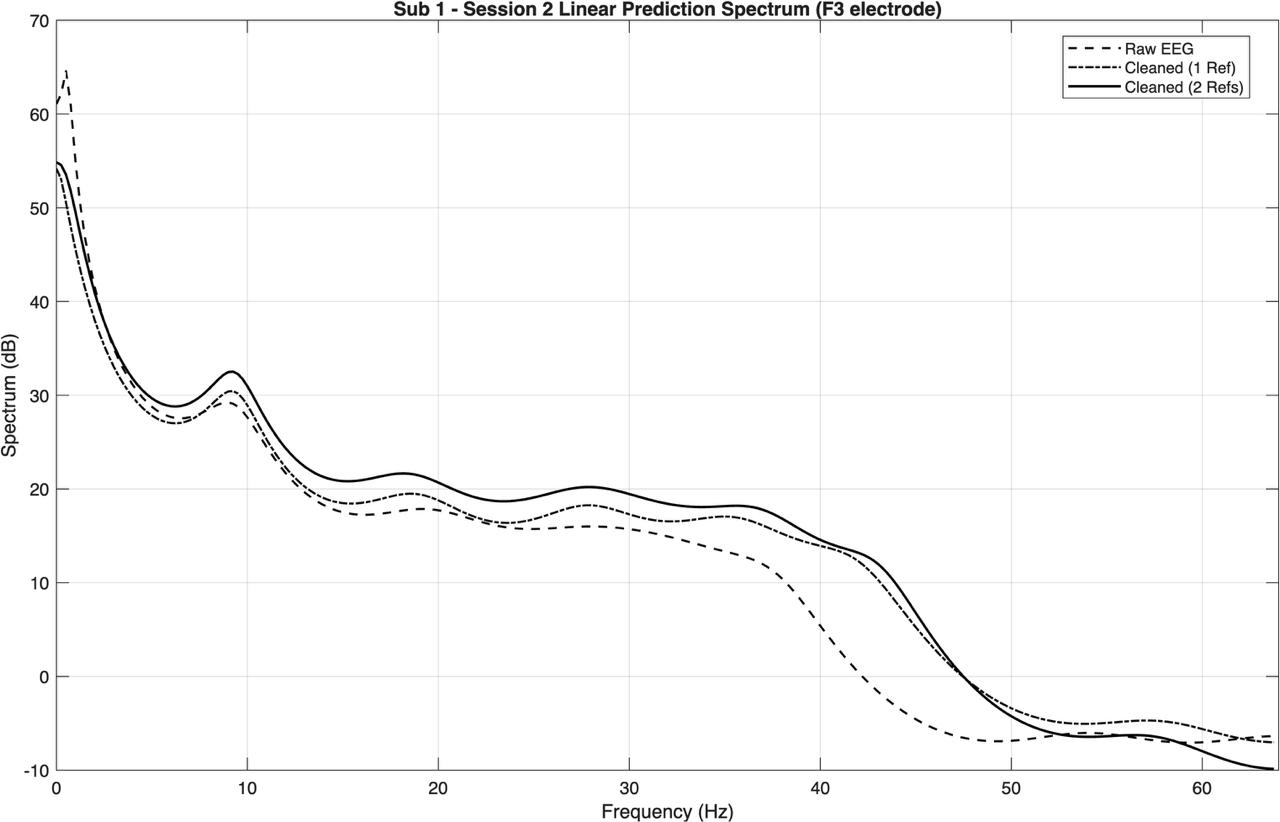
\includegraphics[width=\textwidth]{lp2f3.jpg}
\caption{LP Spectrum Session 2 (F3)}
\end{subfigure}
\hfill
\begin{subfigure}{0.495\textwidth}
\centering
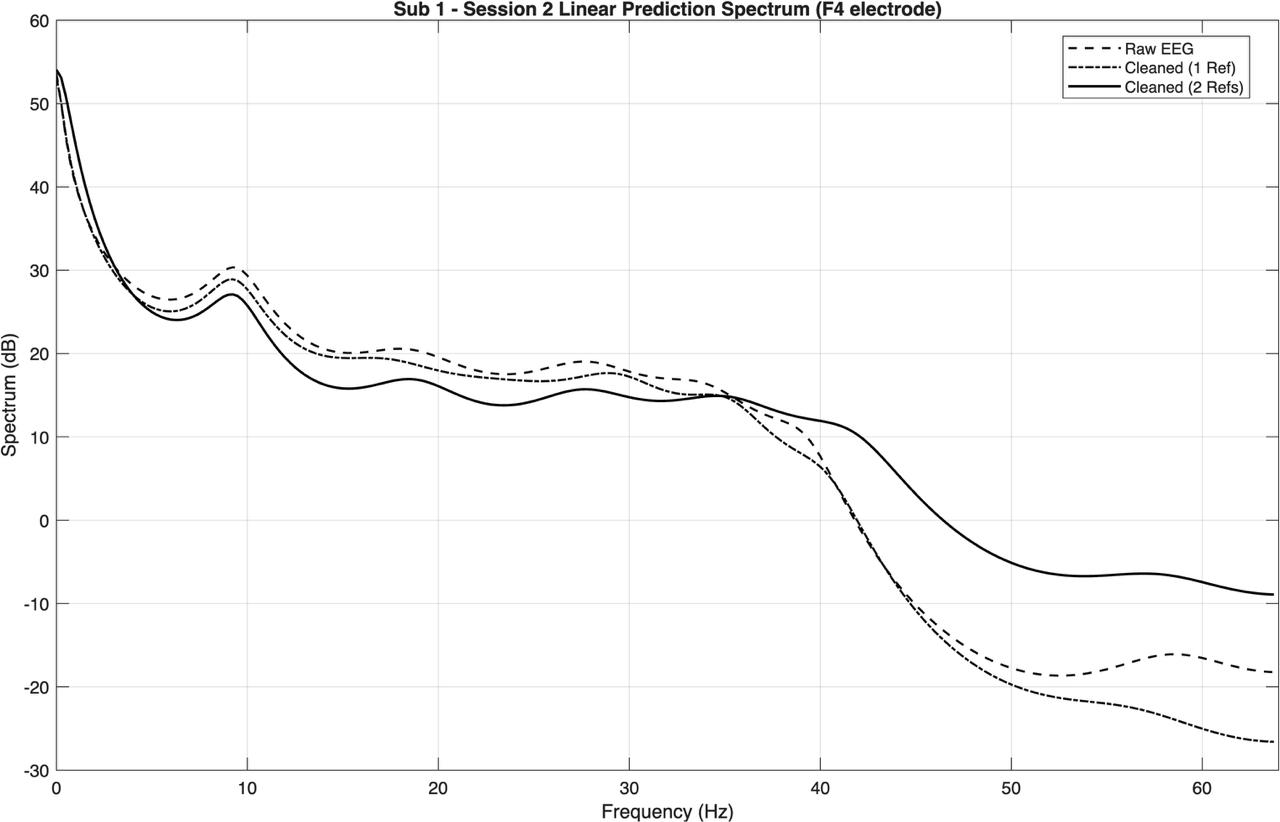
\includegraphics[width=\textwidth]{lp2f4.jpg}
\caption{LP Spectrum Session 2 (F4)}
\end{subfigure}

\caption{Additional LP spectral comparisons for F3 and F4 channels.}
\label{fig:additional_lp_1_2}
\end{figure}

\begin{figure}[H]
\centering
\begin{subfigure}{0.495\textwidth}
\centering
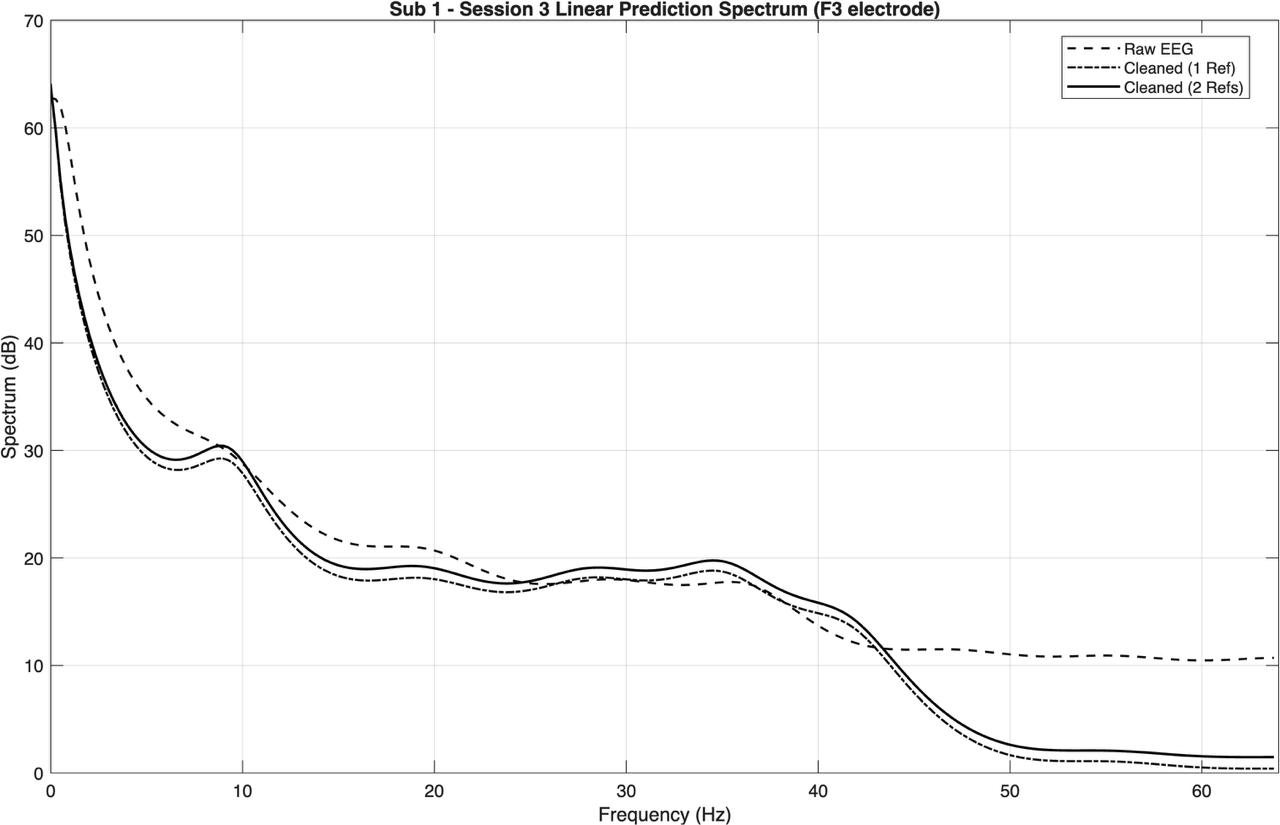
\includegraphics[width=\textwidth]{lp3f3.jpg}
\caption{LP Spectrum Session 3 (F3)}
\end{subfigure}
\hfill
\begin{subfigure}{0.495\textwidth}
\centering
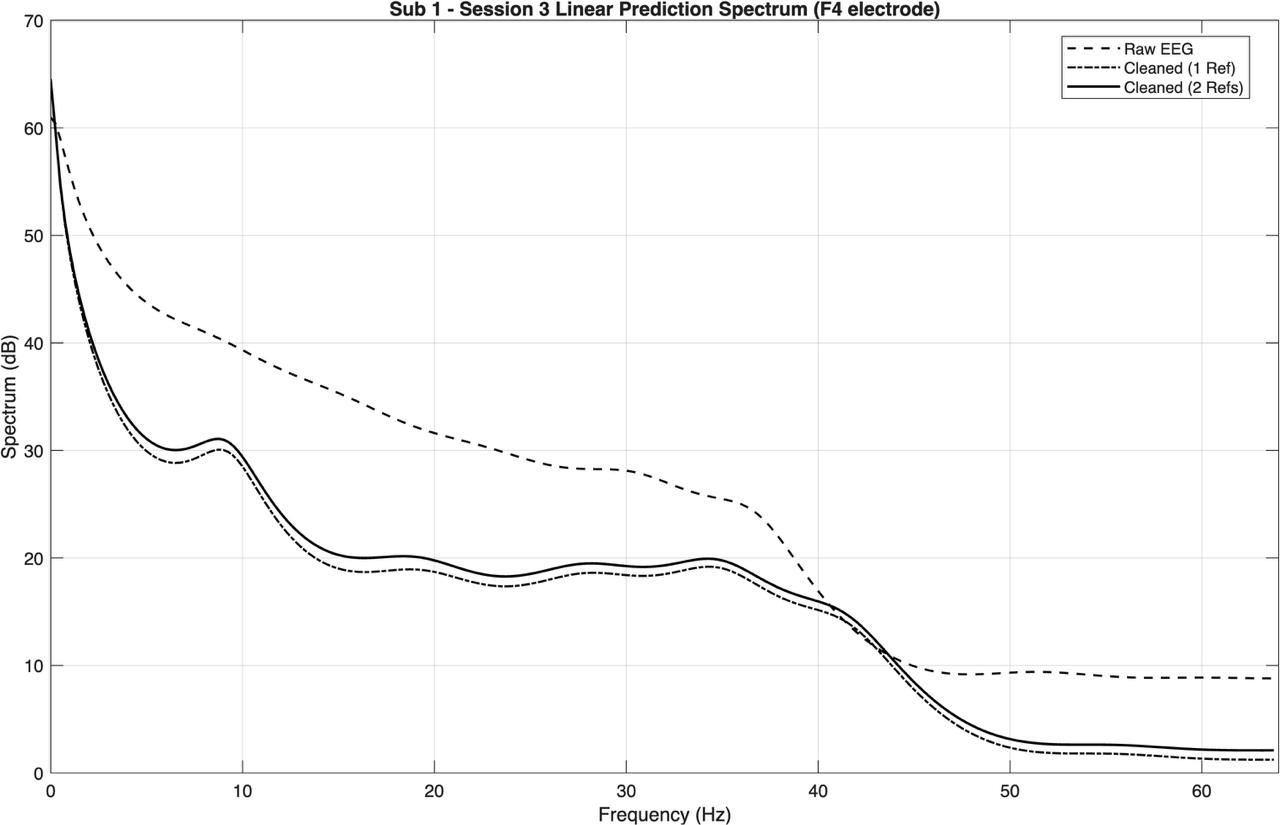
\includegraphics[width=\textwidth]{lp3f4.jpg}
\caption{LP Spectrum Session 3 (F4)}
\end{subfigure}

\vspace{0.4cm}

\begin{subfigure}{0.495\textwidth}
\centering
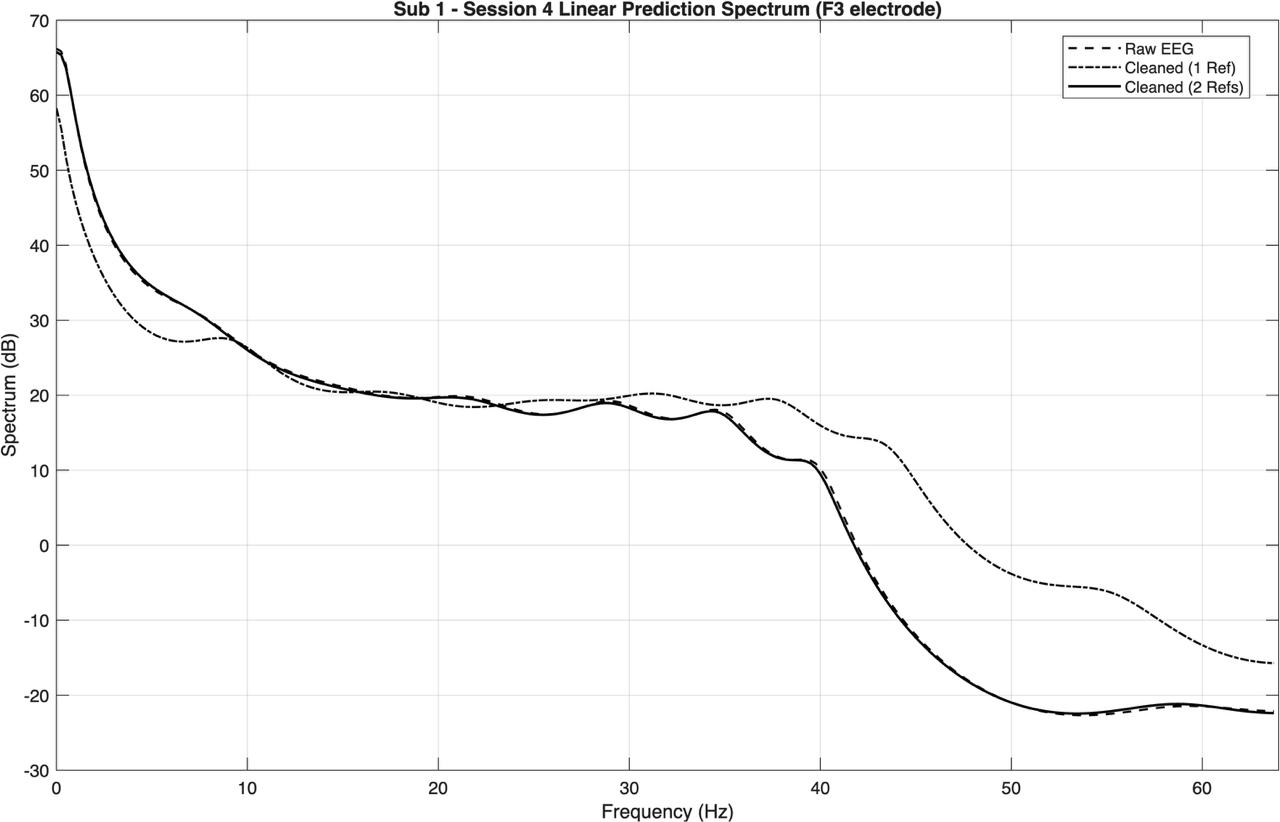
\includegraphics[width=\textwidth]{lp4f3.jpg}
\caption{LP Spectrum Session 4 (F3)}
\end{subfigure}
\hfill
\begin{subfigure}{0.495\textwidth}
\centering
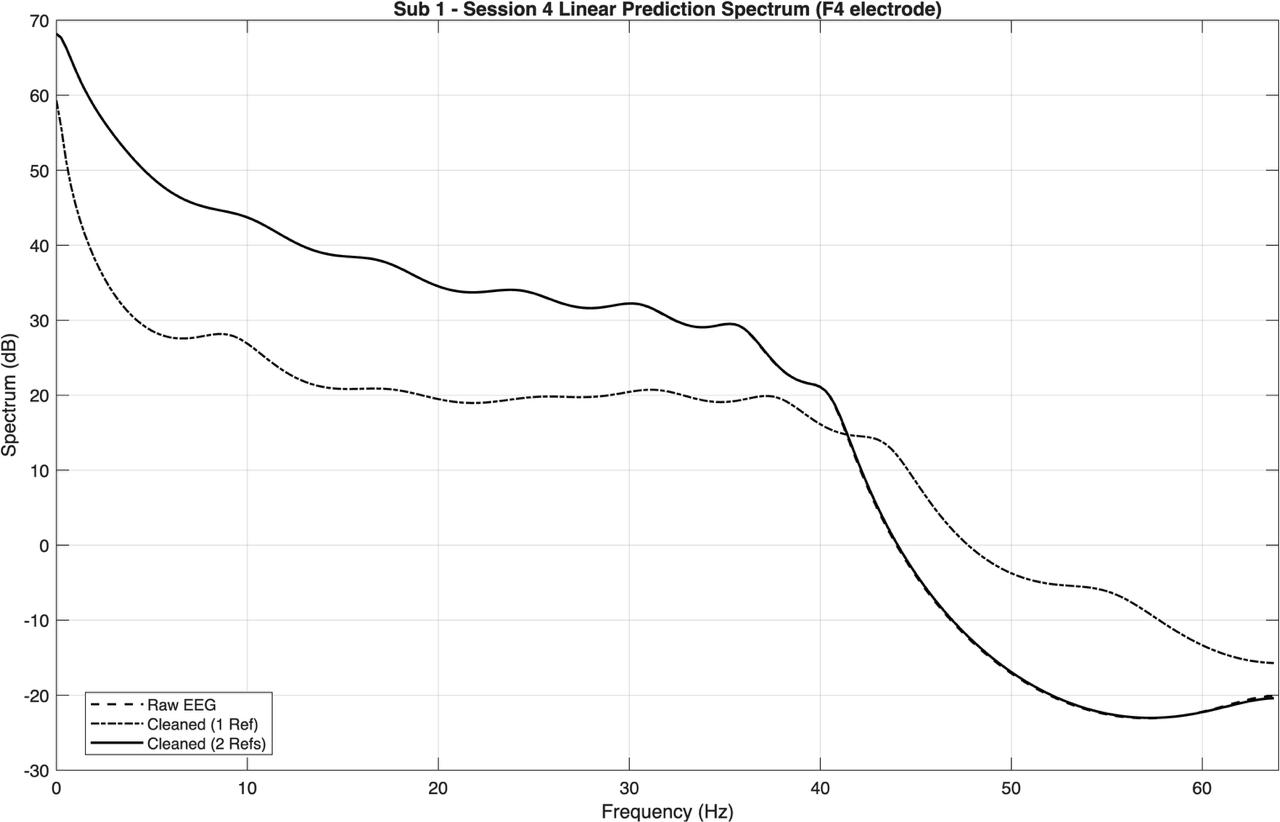
\includegraphics[width=\textwidth]{lp4f4.jpg}
\caption{LP Spectrum Session 4 (F4)}
\end{subfigure}

\caption{Additional LP spectral comparisons for F3 and F4 channels.}
\label{fig:additional_lp_3_4}
\end{figure}

\begin{figure}[H]
\centering
\begin{subfigure}{0.495\textwidth}
\centering
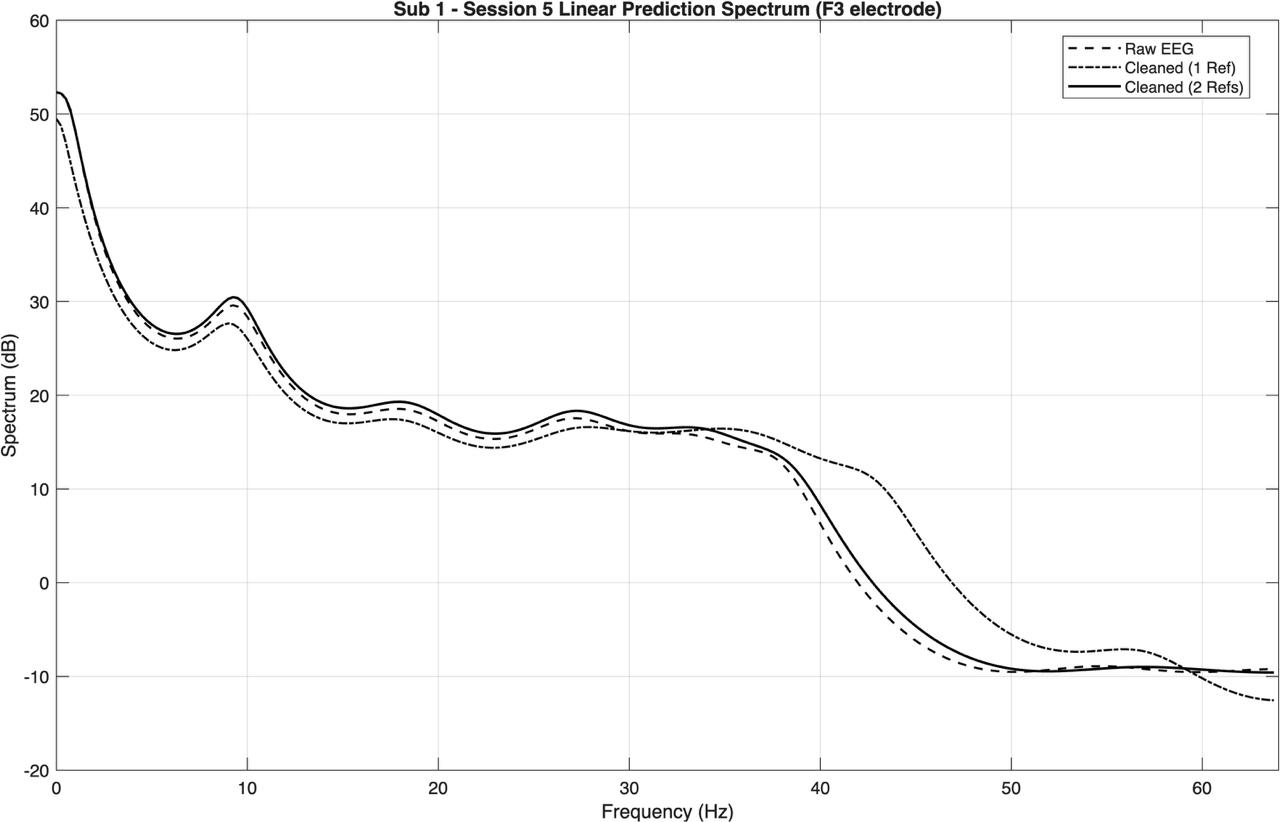
\includegraphics[width=\textwidth]{lp5f3.jpg}
\caption{LP Spectrum Session 5 (F3)}
\end{subfigure}
\hfill
\begin{subfigure}{0.495\textwidth}
\centering
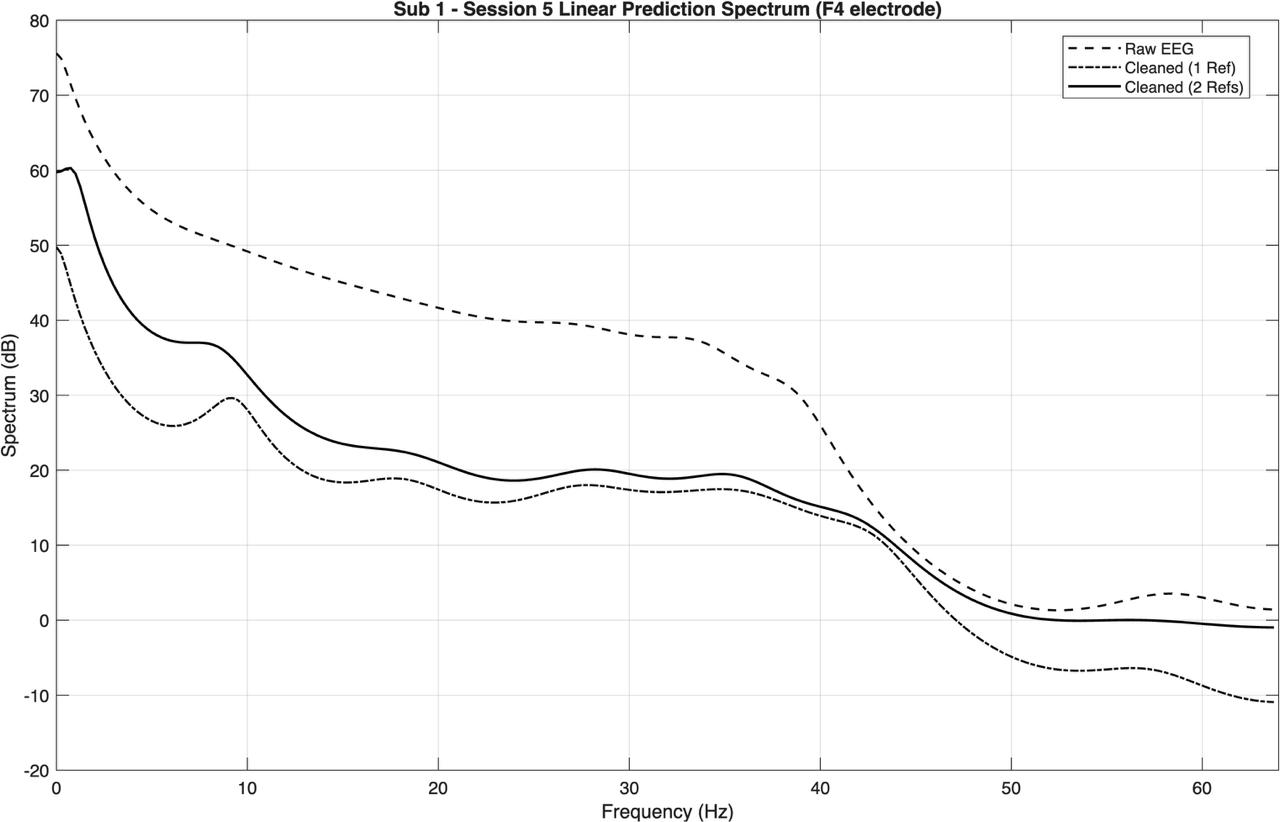
\includegraphics[width=\textwidth]{lp5f4.jpg}
\caption{LP Spectrum Session 5 (F4)}
\end{subfigure}

\vspace{0.4cm}

\begin{subfigure}{0.495\textwidth}
\centering
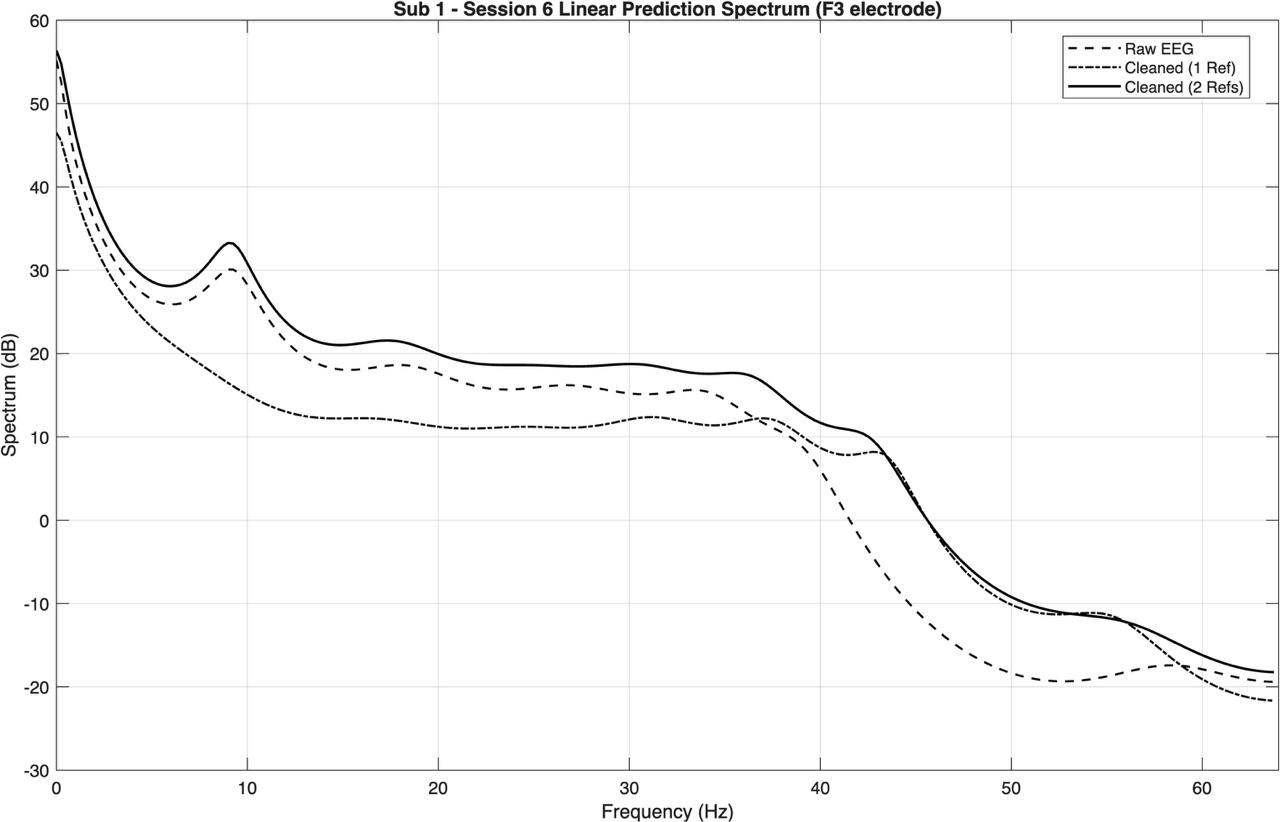
\includegraphics[width=\textwidth]{lp6f3.jpg}
\caption{LP Spectrum Session 6 (F3)}
\end{subfigure}
\hfill
\begin{subfigure}{0.495\textwidth}
\centering
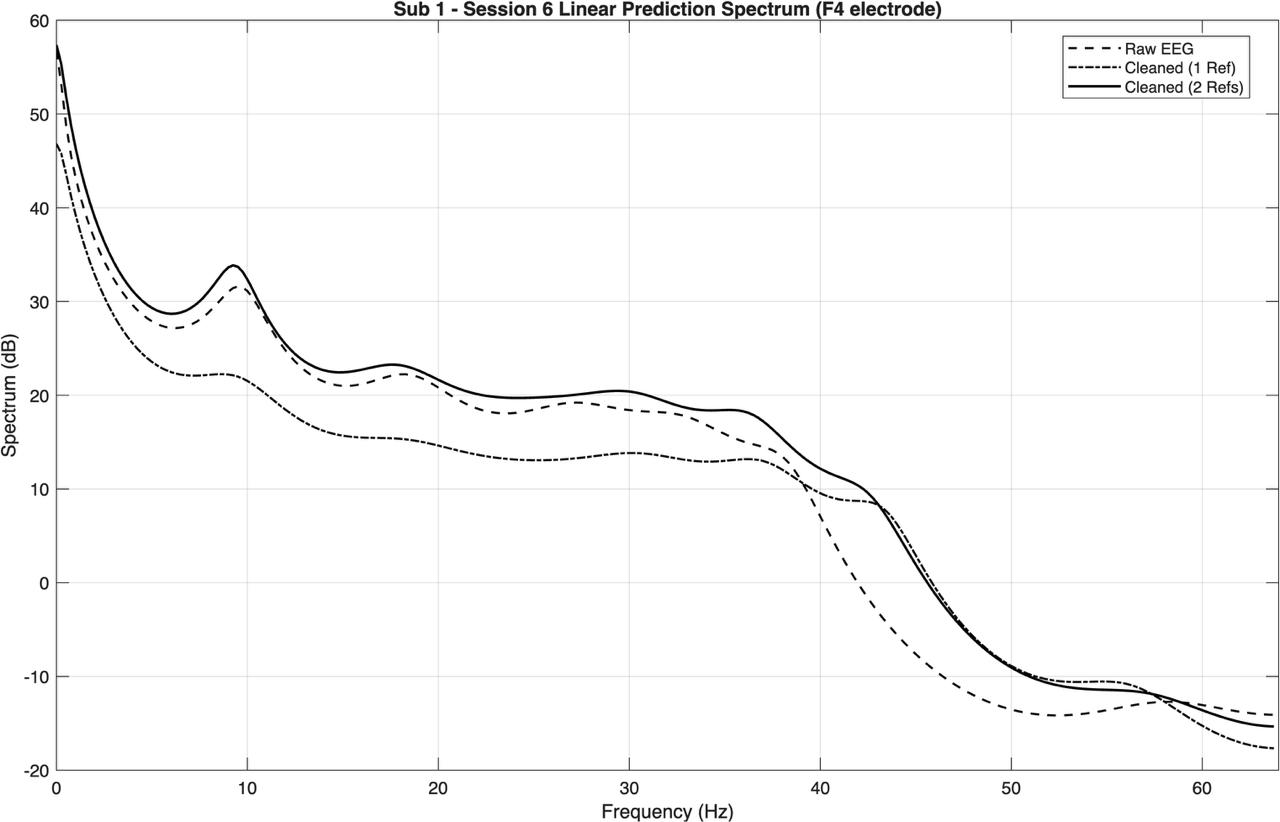
\includegraphics[width=\textwidth]{lp6f4.jpg}
\caption{LP Spectrum Session 6 (F4)}
\end{subfigure}

\caption{Additional LP spectral comparisons for F3 and F4 channels.}
\label{fig:additional_lp_5_6}
\end{figure}

\section{Conclusion}

In this study, Singular Value Decomposition (SVD) was successfully implemented to
mitigate ocular artifacts from recorded EEG signals. The fundamental premise of this
methodology relies on the mathematical principle that neural EEG signals and
electrooculogram (EOG) artifacts occupy distinct orthogonal subspaces, thereby
enabling their structural separation via SVD. For the practical implementation, raw
EEG data recorded from the F3 and F4 frontal electrodes were analyzed in
conjunction with the AF3 and AF4 electrodes, which served as dedicated EOG
reference channels.

The contaminated multi-channel EEG recordings were processed within a custom
MATLAB framework. By constructing observation matrices and applying SVD, the
dominant singular components---which primarily map to high-amplitude EOG
artifacts---were systematically identified and discarded. The underlying EEG signals
were then accurately reconstructed from the remaining lower-energy subspace,
yielding neural data with significantly reduced ocular contamination.

The robustness and efficacy of this proposed approach were rigorously validated
through comprehensive time-domain evaluations and Linear Prediction (LP) spectral
analyses. The time-domain results clearly demonstrated substantial suppression of
large-amplitude ocular spikes, while spectral comparisons confirmed a marked
reduction in low-frequency EOG power without compromising or distorting the
intrinsic neural characteristics in higher frequency bands. Furthermore, the
application of this method across multiple independent EEG datasets yielded
consistently reproducible improvements. Consequently, this study establishes that
the SVD-based technique provides a highly effective, computationally efficient, and
robust framework for isolating and recovering high-fidelity EEG signals from
artifact-contaminated recordings.

\section*{References}

[1] P. K. Sadasivan and D. N. Dutt, "Removal of EOG artifacts from EEG signals using
singular value decomposition," \textit{IEEE Transactions on Biomedical Engineering}, vol. 43,
no. 9, pp. 922--930, 1996.

[2] S. Sanei and J. A. Chambers, \textit{EEG Signal Processing}. John Wiley \& Sons, 2007.

[3] A. Hyvärinen, J. Karhunen, and E. Oja, \textit{Independent Component Analysis}. John
Wiley \& Sons, 2001.

[4] J. A. Urigüen and B. Garcia-Zapirain, "EEG artifact removal---state-of-the-art and
guidelines," \textit{Journal of Neural Engineering}, vol. 12, no. 3, 2015.

[5] M. Fatourechi, A. Bashashati, R. K. Ward, and G. E. Birch, "EMG and EOG artifacts
in brain computer interface systems: A survey," \textit{Clinical Neurophysiology}, vol. 118, no.
3, pp. 480--494, 2007.
\end{document}

